\def\urlSite{https://brevet.initiation.aero}

\newcommand{\iaAssisted}{\fawsomeIa~assisté par IA}

\ifdefined\activerhandout 
\documentclass[12pt,aspectratio=1610,handout]{beamer}
\else
\documentclass[12pt,aspectratio=1610]{beamer}
\fi

\usepackage[
    backend=biber,
    %style=authoryear-icomp,
    style=numeric,
    %style=ieee,
    sortlocale=fr_FR,
    natbib=true,
    url=true, 
    doi=true,
    eprint=true
]{biblatex}

% Le titre et la référence du livre du chapitre restent accessibles à l'image.
\DeclareDataInheritance{inbook}{misc}{%
    \inherit{title}{usera}
    \inherit{crossref}{userb}
}

% Conserver le pilote du style courant pour les autres entrées @misc.
\csletcs{blx@bbx@miscstandard}{blx@bbx@misc}
\DeclareBibliographyDriver{misc}{%
    \iffieldequalstr{entrysubtype}{imageextrait}
        {%
            \iffieldundef{usera}
                {\PackageError{biblio}{Titre du chapitre absent pour \thefield{entrykey}}{Vérifier le crossref vers une entrée inbook avec un titre.}}
                {}%
            \iffieldundef{userb}
                {\PackageError{biblio}{Référence du livre absente pour \thefield{entrykey}}{Vérifier le crossref du chapitre vers le livre.}}
                {}%
            \usebibmacro{bibindex}%
            \usebibmacro{begentry}%
            \printnames{author}%
            \setunit{\addcomma\space}%
            \printfield{title}%
            \setunit{\addcomma\space}%
            \printtext{extrait de \cite{\thefield{userb}}}%
            \setunit{\addcomma\space}%
            \printfield{usera}%
            \setunit{\addcomma\space}%
            \printfield{pages}%
            \newunit\newblock
            \usebibmacro{bytranslator+others}%
            \usebibmacro{finentry}%
        }
        {\csuse{blx@bbx@miscstandard}}%
}

	\addbibresource{commun/biblio.bib}
	\addbibresource{01-EtudeAeronefs/biblio.bib}
	\addbibresource{02-Navigation/biblio.bib}
	\addbibresource{03-Meteo/biblio.bib}
	\addbibresource{04-Aerodynamique/biblio.bib}
	\addbibresource{05-Histoire/biblio.bib}
	\addbibresource{Annexes/biblio.bib}
	\addbibresource{Annexes/friseChronologique/biblio.bib}
	\addbibresource{Annexes/friseChronologique/extraitsVideo/biblio.bib}
	\addbibresource{imgPresentations/biblio.bib}
	\addbibresource{fonts/biblio.bib}
	\addbibresource{fonts/fonts.bib}

%\usepackage[french]{babel} %=> erreur avec les tikz du moteur
\usepackage[T1]{fontenc}
\usepackage[utf8]{inputenc}
\usepackage{lmodern}
\usepackage{hyperref}
\usepackage{smartdiagram}
\usepackage{xcolor}
\usepackage{tikz}
\usepackage{animate}
\usepackage{tikzpeople}
\usepackage{appendixnumberbeamer}
\usepackage[labelformat=empty]{caption}
%\usepackage{pictochrono}
\usepackage{fontawesome5}
\usepackage{awesomebox}
\usepackage{siunitx}
\usepackage{icomma}
\usepackage{physics}
\usepackage[pdftex,outline]{contour} % glow around text
\usepackage{ifthen}
\usepackage{fp}
\usepackage{textcomp}
\usepackage{gensymb}
%Utilisation de police personalisée => compiler avec LuaLaTeX
\ifluatex
\usepackage{fontspec,iftex}
\ifdefined\opendys 
	%Utilisation de la police OpenDyslexic
 	\setmainfont{OpenDyslexic-Regular}[
    		Path = fonts/,  % Chemin du fichier de police
    		Extension = .otf,  % Extension du fichier
    		UprightFont = OpenDyslexic-Regular,  % Utiliser ce fichier pour le texte normal
    		BoldFont = OpenDyslexic-Bold,
    		ItalicFont = OpenDyslexic-Italic,
    		BoldItalicFont = OpenDyslexic-Bold-Italic
	]
	\renewcommand*{\glstextformat}[1]{\textbf{\fontspec{OpenDyslexic-Regular}[
    		Path = fonts/,  % Chemin du fichier de police
    		Extension = .otf,  % Extension du fichier
    		UprightFont = OpenDyslexic-Regular,  % Utiliser ce fichier pour le texte normal
    		BoldFont = OpenDyslexic-Bold,
    		ItalicFont = OpenDyslexic-Italic,
    		BoldItalicFont = OpenDyslexic-Bold-Italic
	]#1}}
\fi	

\newfontfamily\MaterialDesignIcons{Material Design Icons}[
  Path = fonts/,
  Extension = .ttf,
  UprightFont = materialdesignicons-webfont,
  Renderer = OpenType
]
\DeclareTextFontCommand{\mdi}{\MaterialDesignIcons}

\newfontfamily\FontAwsome{Font Awsome Icons}[
  Path = fonts/,
  Extension = .otf,
  UprightFont = FontAwesome7Free-Solid-900,
  Renderer = OpenType
]
\DeclareTextFontCommand{\fawsome}{\FontAwsome}
\fi

\newcommand{\mdiAirBalloon}{\Huge\ifluatex\mdi{ ^^^^^^0f001c }\else\faQuestion\fi\normalsize}
\newcommand{\mdiParachute}{\Huge\ifluatex\mdi{ ^^^^^^0f0cb4 }\else\faQuestion\fi\normalsize}
\newcommand{\mdiRocket}{\Huge\ifluatex\mdi{ ^^^^^^0f14de }\else\faRocket\fi\normalsize}
\newcommand{\mdiBrevet}{\Huge\ifluatex\mdi{ ^^^^^^0f1188 }\else\faCertificate\fi\normalsize}
\newcommand{\mdiTrophy}{\Huge\ifluatex\mdi{ ^^^^^^0f0538 }\else\faTrophy\fi\normalsize}
\newcommand{\mdiMilitaire}{\Huge\ifluatex\mdi{ ^^^^^^0f0787 }\else\faShield\fi\normalsize}
\newcommand{\mdiFemale}{\Huge\ifluatex\mdi{ ^^^^^^0f029c }\else\faFemale\fi\normalsize}
\newcommand{\mdiGreen}{\Huge\ifluatex\mdi{ ^^^^^^0f032a }\else\faLeaf\fi\normalsize}
\newcommand{\mdiSpaceStation}{\Huge\ifluatex\mdi{ ^^^^^^0f1383 }\else\faQuestion\fi\normalsize}

\newcommand{\fawsomeQuestion}{\Huge\ifluatex\fawsome{ ^^^^^^00f059 }\else\faQuestionCircle\fi\normalsize}
\newcommand{\fawsomeAlerte}{\Huge\ifluatex\fawsome{ ^^^^^^00f06a }\else\faExclamationCircle\fi\normalsize}


\usetheme{Warsaw}
\setbeamertemplate{page number in head/foot}[totalframenumber]

\newcommand{\anglais}[1]{(\textit{\color{blue}#1})}
\newcommand{\legende}[2]{\caption{#1\ifdefined\activerbibliobeamer \cite{#2}\fi}}
\newcommand{\histoire}[1]{\begin{awesomeblock}{2pt}{\fawsomeHistoire}{black!75}#1\end{awesomeblock}}
\newcommand{\info}[1]{\begin{awesomeblock}{2pt}{\fawsomeInfo}{blue!75}#1\end{awesomeblock}}
\newcommand{\question}[1]{\begin{awesomeblock}{2pt}{\fawsomeQuestion}{black!75}#1\end{awesomeblock}}
\newcommand{\alerte}[1]{\begin{awesomeblock}{2pt}{\fawsomeAlerte}{red!75}#1\end{awesomeblock}}
\newcommand{\astuce}[1]{\begin{awesomeblock}{2pt}{\fawsomeAstuce}{black!75}#1\end{awesomeblock}}
\newcommand{\exemple}[1]{\begin{awesomeblock}{2pt}{\fawsomeExemple}{black!75}#1\end{awesomeblock}}
\newcommand{\definitionAConnaitre}[1]{\begin{awesomeblock}{2pt}{\fawsomeDefinition}{black!75}#1\end{awesomeblock}}

%\newcommand{\qmcBia}[8]{
%%1 : titre slide
%%2 : numéro de la bonne réponse
%%3 : Inititulé de la question
%%4, 5, 6, et 7 : propositions de réponse
%%8 : explication
%\begin{frame}{#1}
%\begin{awesomeblock}{2pt}{\faQuestion}{black!75}
%#3
%	\begin{enumerate}
%	\ifnum#2=1
%		\only<1>{\item #4}
%		\only<2>{\item \textbf{#4}}
%	\else
%		\item #4
%	\fi
%	\ifnum#2=2
%		\only<1>{\item #5}
%		\only<2>{\item \textbf{#5}}
%	\else
%		\item #5
%	\fi
%	\ifnum#2=3
%		\only<1>{\item #6}
%		\only<2>{\item \textbf{#6}}
%	\else
%		\item #6
%	\fi
%	\ifnum#2=4
%		\only<1>{\item #7}
%		\only<2>{\item \textbf{#7}}
%	\else
%		\item #7
%	\fi
%	\end{enumerate}
%	\pause
%\end{awesomeblock}
%#8
%\end{frame}
%}

\newcommand{\qmcBia}[8]{
%1 : titre slide
%2 : numéro de la bonne réponse
%3 : Inititulé de la question
%4, 5, 6, et 7 : propositions de réponse
%8 : explication
\begin{frame}{#1}
\begin{awesomeblock}{2pt}{\fawsomeQuestionSimple}{black!75}
#3
	\begin{enumerate}
	\item #4
	\item #5
	\item #6
	\item #7
	\end{enumerate}
\end{awesomeblock}
\end{frame}

\begin{frame}{#1}
\begin{awesomeblock}{2pt}{\fawsomeQuestionSimple}{black!75}
#3
	\begin{enumerate}
	\ifnum#2=1
		\item \textbf{#4}
	\else
		\item #4
	\fi
	\ifnum#2=2
		\item \textbf{#5}
	\else
		\item #5
	\fi
	\ifnum#2=3
		\item \textbf{#6}
	\else
		\item #6
	\fi
	\ifnum#2=4
		\item \textbf{#7}
	\else
		\item #7
	\fi
	\end{enumerate}
\end{awesomeblock}
#8
\end{frame}
}

\subtitle{BIA - Brevet d'Initiation Aéronautique}
%\author[BIA]{Clément \textsc{Vermot-Desroches}}
\author[BIA]{\urlSite}
\institute{Collège Aliénor d'Aquitaine\\Martignas-sur-Jalle}
%\date{\today}
\date{Année 2026-2027}

\AtBeginSection[]
{
    \begin{frame}
        %\frametitle{Table of Contents}
        \tableofcontents[currentsection]
    \end{frame}
}

\AtBeginSubsection[]
{
    \begin{frame}
        %\frametitle{Table of Contents}
        \tableofcontents[currentsection,currentsubsection]
    \end{frame}
}

%%%%%%%%%%%%%%%%%%%%%%%%%%%%%%%%%%%%%%%%%%%%%%%%%%%%%%%%%%%%%%%%%%%%%%%%%%%%%%
% \embedvideo{<poster or text>}{<video file (MP4+H264)>}
% \embedvideo*{...}{...}                     % auto-play
%%%%%%%%%%%%%%%%%%%%%%%%%%%%%%%%%%%%%%%%%%%%%%%%%%%%%%%%%%%%%%%%%%%%%%%%%%%%%%
\usepackage[bigfiles]{pdfbase}
\ExplSyntaxOn
\NewDocumentCommand\embedvideo{smm}{
  \group_begin:
  \leavevmode
  \tl_if_exist:cTF{file_\file_mdfive_hash:n{#3}}{
    \tl_set_eq:Nc\video{file_\file_mdfive_hash:n{#3}}
  }{
    \IfFileExists{#3}{}{\GenericError{}{File~`#3'~not~found}{}{}}
    \pbs_pdfobj:nnn{}{fstream}{{}{#3}}
    \pbs_pdfobj:nnn{}{dict}{
      /Type/Filespec/F~(#3)/UF~(#3)
      /EF~<</F~\pbs_pdflastobj:>>
    }
    \tl_set:Nx\video{\pbs_pdflastobj:}
    \tl_gset_eq:cN{file_\file_mdfive_hash:n{#3}}\video
  }
  %
  \pbs_pdfobj:nnn{}{dict}{
    /Type/RichMediaInstance/Subtype/Video
    /Asset~\video
    /Params~<</FlashVars (
      source=#3&
      skin=SkinOverAllNoFullNoCaption.swf&
      skinAutoHide=true&
      skinBackgroundColor=0x5F5F5F&
      skinBackgroundAlpha=0.75
    )>>
  }
  %
  \pbs_pdfobj:nnn{}{dict}{
    /Type/RichMediaConfiguration/Subtype/Video
    /Instances~[\pbs_pdflastobj:]
  }
  %
  \pbs_pdfobj:nnn{}{dict}{
    /Type/RichMediaContent
    /Assets~<<
      /Names~[(#3)~\video]
    >>
    /Configurations~[\pbs_pdflastobj:]
  }
  \tl_set:Nx\rmcontent{\pbs_pdflastobj:}
  %
  \pbs_pdfobj:nnn{}{dict}{
    /Activation~<<
      /Condition/\IfBooleanTF{#1}{PV}{XA}
      /Presentation~<</Style/Embedded>>
    >>
    /Deactivation~<</Condition/PI>>
  }
  %
  \hbox_set:Nn\l_tmpa_box{#2}
  \tl_set:Nx\l_box_wd_tl{\dim_use:N\box_wd:N\l_tmpa_box}
  \tl_set:Nx\l_box_ht_tl{\dim_use:N\box_ht:N\l_tmpa_box}
  \tl_set:Nx\l_box_dp_tl{\dim_use:N\box_dp:N\l_tmpa_box}
  \pbs_pdfxform:nnnnn{1}{1}{}{}{\l_tmpa_box}
  %
  \pbs_pdfannot:nnnn{\l_box_wd_tl}{\l_box_ht_tl}{\l_box_dp_tl}{
    /Subtype/RichMedia
    /BS~<</W~0/S/S>>
    /Contents~(embedded~video~file:#3)
    /NM~(rma:#3)
    /AP~<</N~\pbs_pdflastxform:>>
    /RichMediaSettings~\pbs_pdflastobj:
    /RichMediaContent~\rmcontent
  }
  \phantom{#2}
  \group_end:
}
\ExplSyntaxOff
%%%%%%%%%%%%%%%%%%%%%%%%%%%%%%%%%%%%%%%%%%%%%%%%%%%%%%%%%%%%%%%%%%%%%%%%%%%%%%

\usetikzlibrary{calc,fit}
\tikzset{>=latex} % for LaTeX arrow head
\colorlet{knob}{blue!20!black!40}
\colorlet{mylightblue}{blue!10}
\colorlet{mydarkblue}{blue!30!black}
\tikzstyle{arrow}=[<-,very thick,mydarkblue]
\tikzstyle{vector}=[->,line width=2,green!50!black]

% ANGLE
\newcommand{\getangle}[3]{%
    \pgfmathanglebetweenpoints{\pgfpointanchor{#2}{center}}
                              {\pgfpointanchor{#3}{center}}
    \global\let#1\pgfmathresult  
}

\newcommand{\echelleTikz}{1.0}

% ENGINE
\def\gas{blue!10}
\def\engine#1{
  \def\R{2}
  \def\l{1}
  \def\L{4.6}
  \def\p{1.8}
  \def\P{3.2}
  \def\Ra{.35} % crankshaft
  \def\Rb{.6}  % crankshaft
  \def\Rc{.2}  % crankshaft
  \def\a{40} % wall
  \def\b{30} % rod
  \coordinate (O)   at (0,0);
  \coordinate (CS)  at (#1:\l);
  \coordinate (P)   at (0,{\l*sin(#1)+sqrt(\P^2-(\l*cos(#1))^2)});
  \coordinate (RL)  at (180-\a:\R);
  \coordinate (RR)  at (\a:\R);
  \coordinate (TL)  at ($(RL)+(0,\L)$);
  \coordinate (TR)  at ($(RR)+(0,\L)$);
  \coordinate (T)   at ($(TL)!.5!(TR)$);
  \coordinate (PL)  at ($(RL)+(0,{\l*(1.4+sin(#1))})$);
  
  \coordinate (PR)  at ($(PL-|RR)+(0,\p)$);
  \coordinate (S)   at ($(T)+(0,.8)$);
  \coordinate (VLo) at ($(TL)!.2!(S)$);
  \coordinate (VL)  at ($(TL)!.4!(S)$);
  \coordinate (VLm) at ($(TL)!.6!(S)$);
  \coordinate (VRo) at ($(TR)!.2!(S)$);
  \coordinate (VR)  at ($(TR)!.4!(S)$);
  \coordinate (VRm) at ($(TR)!.6!(S)$);
  \getangle{\c}{CS}{P}
  \getangle{\vl}{VLo}{VLm}
  \getangle{\vr}{VRo}{VRm}
  
  % GAS
  \fill[\gas,draw=white,line width=3] (PL) -| (TR) -- (S) -- (TL) -- cycle;
  
  % CRANKSHAFT
  \draw[thick,mydarkblue,top color=blue!30!black!40,bottom color=blue!30!black!10,shading angle=180]
    (O) ++ (180+#1:\Ra) to[out={-90+#1},in={180+#1},looseness=.8]
    ($(CS)+(-90+#1:\Rb)$) arc (-90+#1:90+#1:\Rb) to[out=180+#1,in=90+#1,looseness=.8] cycle;
  
  % ROD
  \draw[thick,mydarkblue,top color=blue!30!black!50,bottom color=blue!30!black!20,shading angle=\c]
    (CS) ++ (\c-\b:\Rb) arc (\c-\b:-360+\c+\b:\Rb) -- ($(P)+(\c+90:\Rc)$) -- ($(P)+(\c-90:\Rc)$) -- cycle;
  
  % PISTON
  \draw[mydarkblue,thick,top color=blue!20!black!30,bottom color=blue!20!black!30,middle color=blue!5,shading angle=90]
    (PL) rectangle (PR);
  \draw[thick,mydarkblue,fill=knob]
    (PL) ++ (0,.70*\p) rectangle ($(PR)+(0,-.25*\p)$);
  \draw[thick,mydarkblue,fill=knob]
    (PL) ++ (0,.59*\p) rectangle ($(PR)+(0,-.46*\p)$);
  
  % DECORATION
  \draw[thick,mydarkblue,fill=knob] (O) circle (\Rc/2);
  \draw[thick,mydarkblue,fill=knob] (CS) circle (\Rc);
  \draw[thick,mydarkblue,fill=knob] (P) circle (\Rc);
  
  % WALL
  \wall
}

% WALL
\def\wall{
  \draw[line width=4,blue!10!black!50]
    (VRo) ++ (1.5,0.6) to[out=180,in=60] (VRo) -- (TR) -- %to[out=-30,in=90,looseness=0.5]
    (RR) arc (\a:-180-\a:\R) --
    (TL) -- (VLo) to[out=110,in=0] ++ (-1.5,0.6); %to[out=90,in=200,looseness=0.8]
  \draw[line width=4,blue!10!black!50]
    (VLo) ++ (-1.5,1.3) to[out=0,in=110] (VLm) -- (S) --
    (VRm) to[out=60,in=180] ($(VRo)+(1.5,1.3)$);
    
  \fill[blue!30!black!60]
    (S) ++ (.07,.2) to[out=90,in=-150]++ (1,1.4) -- ($(S)+(1,1.74)$)
    to[out=-150,in=90] ($(S)+(-.07,.2)$);
  \draw[blue!30!black!80]
    (S) ++ (.07,.2) to[out=90,in=-150]++ (1,1.4)
    (S) ++ (-.07,.2) to[out=90,in=-150]++ (1.07,1.54);
  \draw[blue!10!black,fill=blue!20!black]
    (S) ++ (-.09,-.16) --++ (.09,-.1) coordinate (X) --++ (.09,.1) -- cycle;
  \draw[blue!30!black,fill=blue!30!black!80]
    (S) ++ (-.1,-.15) --++ (.2,0) --++ (0,.35) --++ (-.2,0) -- cycle;
}

% VALVE
\def\valveL#1{
  \fill[thick,blue!20!black]
    (VLo) ++ (\vl-90:#1) -- ($(VLm)+(\vl-90:#1)$) -- ($(VLo)!.64!(VLm)+(\vl+90:.2-#1)$) --++ (\vl+90:2)
    -- ($(VLo)!.36!(VLm)+(\vl+90:2.2-#1)$) -- ($(VLo)!.36!(VLm)+(\vl+90:.2-#1)$) -- cycle;
}

% VALVE
\def\valveR#1{
  \fill[thick,blue!20!black]
    (VRo) ++ (\vr+90:#1) -- ($(VRm)+(\vr+90:#1)$) -- ($(VRo)!.64!(VRm)+(\vr-90:.2-#1)$) --++ (\vr-90:2)
    -- ($(VRo)!.36!(VRm)+(\vr-90:2.2-#1)$) -- ($(VRo)!.36!(VRm)+(\vr-90:.2-#1)$) -- cycle;
}

\title[Séance 3 - Motorisation]{Séance 3 \\ Motorisation}

\usepackage{animate}

\begin{document}
 \begin{frame}
 \titlepage
 \end{frame}
 
 \begin{frame}
 \tableofcontents
 \end{frame}
 
 \section{Le moteur 4 temps}
 \begin{frame}{Le moteur à combustion interne}
	\begin{figure}[H]
  	\only<1| handout:0>{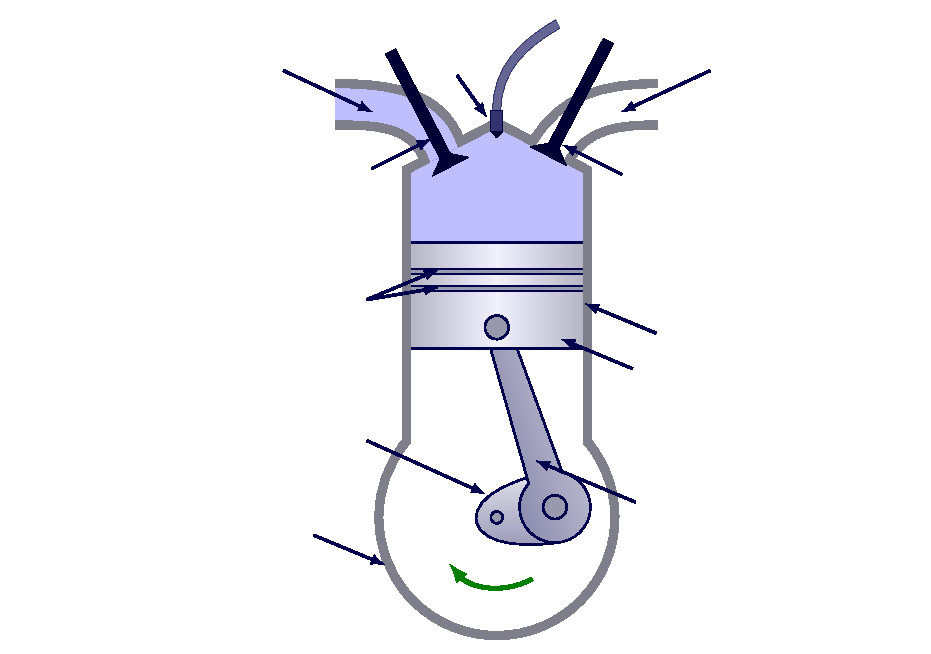
\includegraphics[scale=0.7]{01-EtudeAeronefs/img/Cycle4Temps/0-MoteurLegendeFlechesSeulement_doc.pdf}}
  	\only<2>{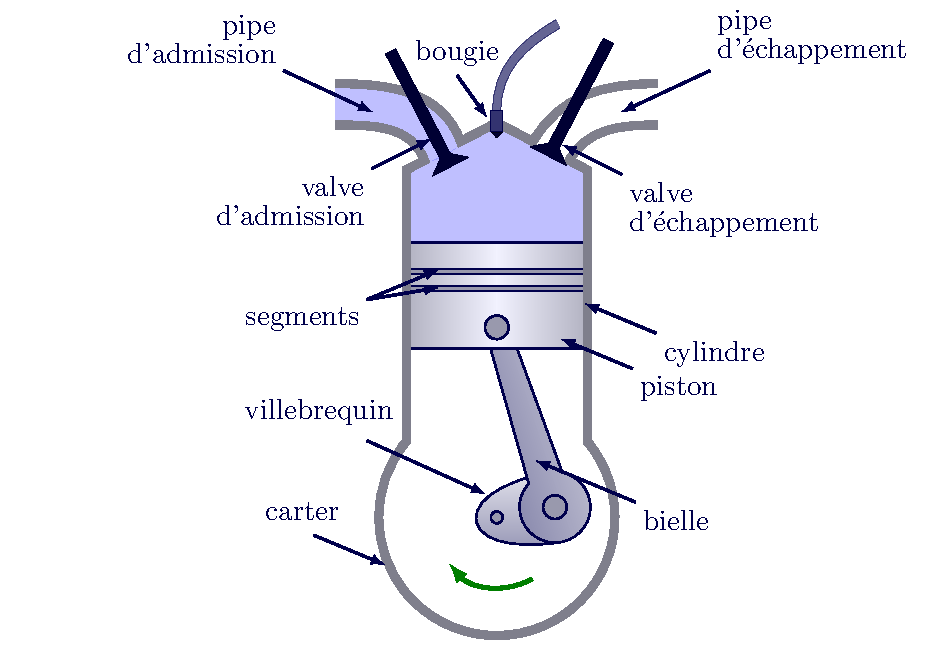
\includegraphics[scale=0.7]{01-EtudeAeronefs/img/Cycle4Temps/0-MoteurLegende_doc.pdf}}
	\end{figure}
	\pause
 \end{frame}
 
 \subsection{Le cycle à 4 temps}
 \begin{frame}{Admission}
 \begin{columns}
 \begin{column}{0.65\textwidth}
 	\only<2>{\begin{itemize}
 		\item La soupape d'admission est ouverte
 		\item Le piston descend
 		\item Le mélange air-carburant est aspiré dans le cylindre
 	\end{itemize}}
 \end{column}
 \begin{column}{0.35\textwidth}
 \begin{figure}[H]
  		\centering
  		\renewcommand{\echelleTikz}{0.5}
  		\scalebox{1.2}{\begin{minipage}{3cm}
		% INTAKE STROKE
\begin{tikzpicture}[scale=\echelleTikz]
  \def\d{-60}
  \engine{10};
  \draw[vector] (\d:.6*\R) arc (\d:\d-80:.55*\R);
  \fill[\gas]
    (VLo) to[out=110,in=0] ++ (-1.5,0.6) -- ($(VLo)+(-1.5,1.3)$) to[out=0,in=110] (VLm) to[out=\vl-90,in=\vl-90] cycle;
  \wall
  \valveL{.3}
  \valveR{.1};
  
\end{tikzpicture}
		\end{minipage}	}	
		\end{figure}
 \end{column}
 \end{columns}
 \pause
 \end{frame} 
 
 \begin{frame}{Compression}
 \begin{columns}
 \begin{column}{0.35\textwidth}
 \begin{figure}[H]
  		\centering
  		\renewcommand{\echelleTikz}{0.5}
  		\scalebox{1.2}{\begin{minipage}{3cm}
		% COMPRESSION STROKE
\def\gas{blue!50}
\begin{tikzpicture}[scale=\echelleTikz]
  \def\d{-10}
  \engine{-140};
  \draw[vector] (\d:.6*\R) arc (\d:\d-80:.55*\R);
  \valveL{.1}
  \valveR{.1}
\end{tikzpicture}
		\end{minipage}	}	
		\end{figure}
 \end{column}
 \begin{column}{0.65\textwidth}
 	\only<2>{\begin{itemize}
 		\item Les soupapes sont fermées
 		\item Le piston remonte
 		\item Le mélange est compressé dans le cylindre.
 	\end{itemize}}
 \end{column}
 \end{columns}
 \pause
 \end{frame} 
 
  \begin{frame}{Explosion-détente}
 \begin{columns}
 \begin{column}{0.65\textwidth}
 	\only<2-4>{\begin{itemize}
 		\item Les soupapes sont fermées
 		\item La bougie produit une étincelle quand le piston est au point haut
 		\item Le piston est repoussé vers le bas par l'explosion
 	\end{itemize}
 	\only<3-4>{\info{Le temps d'explosion-détente est le seul temps qui produit de l'énergie}}
 	\only<4>{\alerte{Un moteur d'avion est généralement équipé de 2 bougies par cylindre pour augmenter la sécurité}}}
 \end{column}
 \begin{column}{0.35\textwidth}
 \begin{figure}[H]
  		\centering
  		\renewcommand{\echelleTikz}{0.5}
  		\scalebox{1.2}{\begin{minipage}{3cm}
		% IGNITION
\def\gas{blue!50}
\begin{tikzpicture}[scale=\echelleTikz]
  \def\d{40}
  \engine{90};
  \draw[vector] (\d:.6*\R) arc (\d:\d-80:.55*\R);
  \valveL{.1}
  \valveR{.1}
  \draw[very thin,yellow!70!black,fill=yellow,shift={(X)}]
    ( -15:.20) -- ( -30:.40) -- ( -40:.25) -- ( -50:.40) --
    ( -60:.22) -- ( -70:.40) -- ( -80:.20) -- ( -90:.45) --
    (-100:.24) -- (-110:.40) -- (-120:.25) -- (-130:.40) --
    (-140:.20) -- (-150:.45) -- (-165:.20) to[out=40,in=140] cycle;
\end{tikzpicture}
		\end{minipage}	}	
		\end{figure}
 \end{column}
 \end{columns}
 \pause
 \pause
 \pause
 \end{frame} 
 
 \begin{frame}{Échappement}
 \begin{columns}
 \begin{column}{0.35\textwidth}
 \begin{figure}[H]
  		\centering
  		\renewcommand{\echelleTikz}{0.5}
  		\scalebox{1.2}{\begin{minipage}{3cm}
		% EXHAUST STROKE
\begin{tikzpicture}[scale=\echelleTikz]
  \def\d{-40}
  \engine{-190};
  \draw[vector] (\d:.6*\R) arc (\d:\d-80:.55*\R);
  \fill[\gas]
    (VRo) to[out=60,in=-180] ++ (1.5,0.6) -- ($(VRo)+(1.5,1.3)$) to[out=180,in=60] (VRm) to[out=-270+\vr,in=-270+\vr] cycle;
  \wall
  \valveL{.1}
  \valveR{.3}
\end{tikzpicture}
		\end{minipage}	}	
		\end{figure}
 \end{column}
 \begin{column}{0.65\textwidth}
 	\only<2>{\begin{itemize}
 		\item La soupape d'échappement s'ouvre
 		\item La remontée du piston chasse les gaz brûlés du cylindre
 	\end{itemize}}
 \end{column}
 \end{columns}
 \pause
 \end{frame}
 
 \begin{frame}{Cycle complet}
 \begin{figure}[H]
  		\centering
  		\renewcommand{\echelleTikz}{0.5}
  		\scalebox{.6}{\begin{minipage}{3cm}
		% Définition des couleurs de base
\definecolor{gazFroid}{RGB}{173,216,230}     % Bleu clair
\definecolor{gazChaud}{RGB}{255,0,0}         % Rouge
\definecolor{gazExplosion}{RGB}{255,255,0}   % Jaune
\definecolor{gazBrule}{RGB}{128,128,128}     % Gris

% Définition des couleurs de base
\definecolor{gazFroid}{RGB}{173,216,230}     % Bleu clair
\definecolor{gazChaud}{RGB}{255,0,0}         % Rouge
\definecolor{gazExplosion}{RGB}{255,255,0}   % Jaune
\definecolor{gazBrule}{RGB}{128,128,128}     % Gris

% Définition de la couleur des gaz en fonction de l'angle
\newcommand{\setGasColor}[1]{%
    \def\angle{#1}%
    % De gris à bleu (-90 à -30)
    \ifnum\angle<-30
        \def\gas{gazBrule!\the\numexpr100-(((\angle+90)*100)/60)\relax!gazFroid}%
    \else
        % Bleu constant (-30 à 90)
        \ifnum\angle<90
            \def\gas{gazFroid}%
        \else
            % De bleu vers rouge (90 à 270)
            \ifnum\angle<270
                \def\gas{gazFroid!\the\numexpr100-((\angle-90)*100/180)\relax!gazChaud}%
            \else
                % De rouge vers jaune (270 à 300)
                \ifnum\angle<300
                    \def\gas{gazChaud!\the\numexpr((\angle-270)*100/30)\relax!gazExplosion}%
                \else
                    % De jaune vers gris (300 à 450)
                    \ifnum\angle<450
                        \def\gas{gazExplosion!\the\numexpr100-((\angle-300)*100/150)\relax!gazBrule}%
                    \else
                        % Gris constant (450 à 630)
                        \def\gas{gazBrule}%
                    \fi
                \fi
            \fi
        \fi
    \fi
}

%\ifdefined\activeranimations 
\newcommand{\nbFramesMoteurAnime}{360}
%\else
%\newcommand{\nbFramesMoteurAnime}{1}
%\fi

\begin{animateinline}[autoplay,loop,controls]{60}
\multiframe{\nbFramesMoteurAnime}{i=-90+2}{%
    \begin{tikzpicture}
    \setGasColor{\i}%
      \coordinate (boiteLegende1) at (0,8.5);
      \coordinate (boiteLegende2) at (0,9);
      \node[rectangle,minimum width=2cm] [fit = (boiteLegende1) (boiteLegende2)] (legende) {};    
    
      \engine{-\i}
      
      % INTAKE STROKE
      \ifnum\i>-92 \ifnum\i<-88 
          \node[align=center,font=\Large] at (legende.center) {\textbf{Admission}};
          \valveL{.2}
          \valveR{.1};
      \fi \fi 
      \ifnum\i>-90 \ifnum\i<90 
          \node[align=center,font=\Large] at (legende.center) {\textbf{Admission}};
          \setGasColor{\i}%
          \fill[\gas, opacity=0.5]
              (VLo) to[out=110,in=0] ++ (-1.5,0.6) -- ($(VLo)+(-1.5,1.3)$) to[out=0,in=110] (VLm) to[out=\vl+5,in=\vl-47] cycle;
          \wall
          \valveL{.3}
          \valveR{.1};
      \fi \fi
      
      % COMPRESSION STROKE
      \ifnum\i>89 \ifnum\i<272 
          \node[align=center,font=\Large] at (legende.center) {\textbf{Compression}};
          \valveL{.1}
          \valveR{.1};
      \fi \fi 
      
      % POWER STROKE
      \ifnum\i>270 \ifnum\i<452 
          \node[align=center,font=\Large] at (legende.center) {\textbf{Explosion-détente}};
          \valveL{.1}
          \valveR{.1};
      \fi \fi
      
      % EXHAUST STROKE
      \ifnum\i>451 \ifnum\i<630
          \node[align=center,font=\Large] at (legende.center) {\textbf{Echappement}};
          \fill[\gas, opacity=0.5]
              (VRo) to[out=60,in=-180] ++ (1.5,0.6) -- ($(VRo)+(1.5,1.3)$) to[out=180,in=60] (VRm) to[out=-220+\vr,in=-180+\vr] cycle;
          \wall 
          \valveL{.1}
          \valveR{.3};
      \fi \fi
      
      % IGNITION
      \ifnum\i>268 \ifnum\i<280 
          \draw[very thin,yellow!70!black,fill=yellow,shift={(X)}]
              ( -15:.20) -- ( -30:.40) -- ( -40:.25) -- ( -50:.40) --
              ( -60:.22) -- ( -70:.40) -- ( -80:.20) -- ( -90:.45) --
              (-100:.24) -- (-110:.40) -- (-120:.25) -- (-130:.40) --
              (-140:.20) -- (-150:.45) -- (-165:.20) to[out=40,in=140] cycle; 
      \fi \fi 
    \end{tikzpicture}
  }
\end{animateinline}
		\end{minipage}	}	
		\end{figure}		
 \end{frame}
 
 \begin{frame}{Système d'allumage}
 \begin{columns}
 \begin{column}{0.5\textwidth}
 	\begin{itemize}
 		\item Double magnéto : améliore la fiabilité
 		\item Double bougie : améliore la combustion
 		\item Sélecteur de magnéto dans le cockpit
 	\end{itemize}
 \end{column}
 \begin{column}{0.5\textwidth}
 	\begin{figure}[H]
  		\centering
    		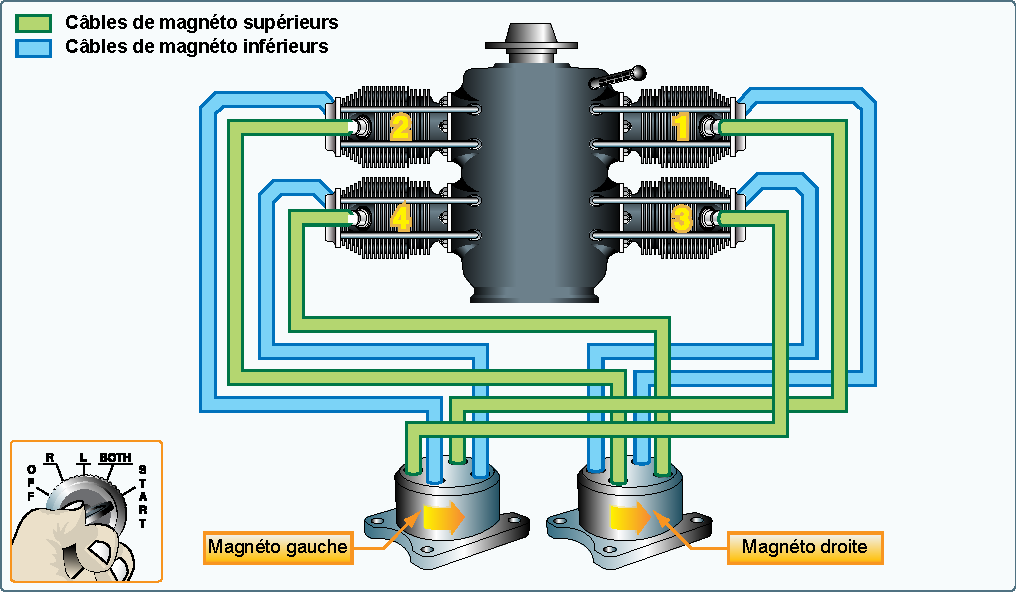
\includegraphics[width=1.07\textwidth]{01-EtudeAeronefs/img/systemesAvion/systemeAllumage.pdf}
  		\legende{Système d'allumage}{img:systemeAllumage}
	\end{figure}	
 \end{column}
 \end{columns}
 \end{frame}
 
 \begin{frame}{Carburateur}
 \begin{columns}
 \begin{column}{0.5\textwidth}
 	\begin{itemize}
 		\item Produit le mélange air-carburant ($1/15^{\text{e}}$)
 		\item Dépression dans le venturi qui provoque la vaporisation du carburant
 	\end{itemize}
 \end{column}
 \begin{column}{0.5\textwidth}
 	\begin{figure}[H]
  		\centering
    		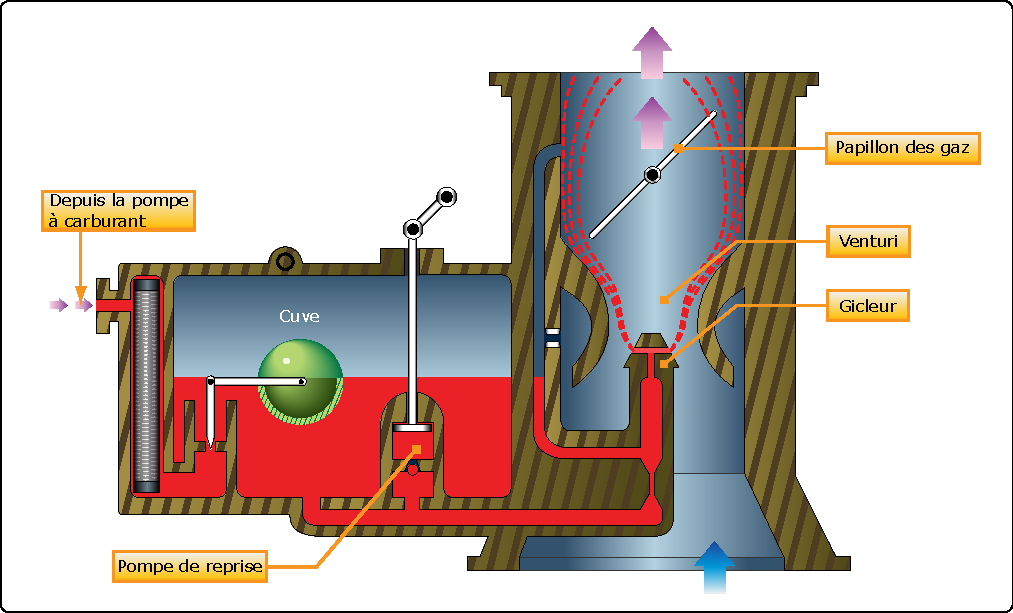
\includegraphics[width=1.07\textwidth]{01-EtudeAeronefs/img/systemesAvion/carburateur.pdf}
  		\legende{Schéma d'un carburateur}{img:carburateur}
	\end{figure}	
 \end{column}
 \end{columns}
 
 \end{frame}
 
  \begin{frame}{Le givrage carburateur}
 \begin{columns}
 \begin{column}{0.5\textwidth}
 	\begin{figure}[H]
  		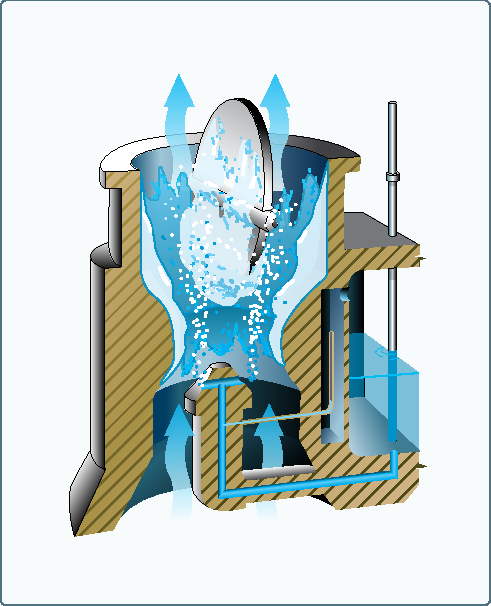
\includegraphics[width=0.75\textwidth]{01-EtudeAeronefs/img/systemesAvion/givrageCarbu.pdf}
  		\legende{Givrage carbu}{img:givrageCarbu}
	\end{figure}	
 \end{column}
 \begin{column}{0.5\textwidth}
 	\begin{itemize}
 		\item La dépression dans le venturi provoque une baisse de la température
 		\item Suffisante pour faire geler l'eau contenue dans l'air
 	\end{itemize}
 	\pause
 	\alerte{Peut provoquer l'arrêt du moteur}
 \end{column}
 
 \end{columns}
 \end{frame}
 
 \begin{frame}{Réchauffage carburateur}
 \begin{figure}[H]
  		\centering
    		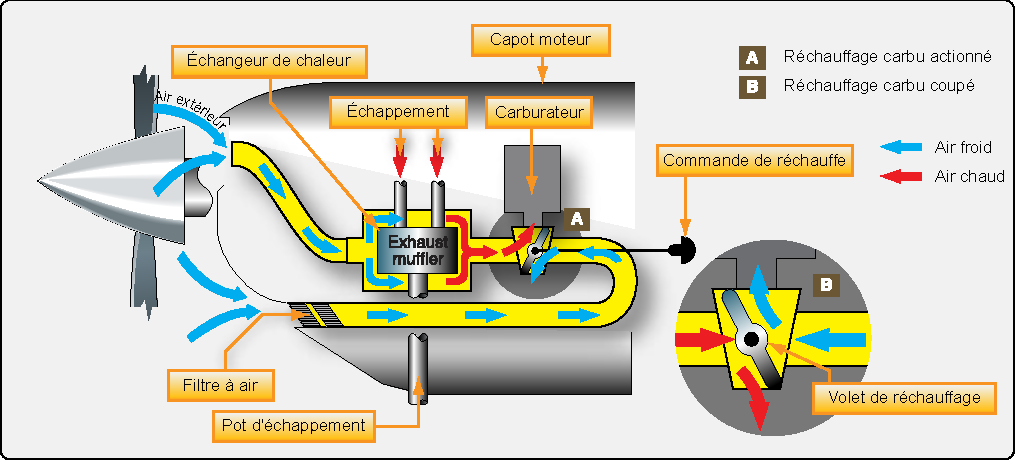
\includegraphics[width=0.75\textwidth]{01-EtudeAeronefs/img/rechauffeCarbu.pdf}
  		\legende{Réchauffage carburateur}{img:rechauffeCarbu}
	\end{figure}	
	\pause
	\alerte{L'usage de la "réchauffe carbu" réduit la puissance délivrée par le moteur (air chaud moins dense)}
 
 \end{frame}
 
 \subsection{Différentes dispositions de cylindres}
 \begin{frame}{Les dispositions de cylindres}
 Afin d'augmenter la puissance des moteurs et d'améliorer la régularité de fonctionnement, les concepteurs des moteurs ont rapidement multiplié le nombre de cylindres de leurs moteurs.
 
 \question{Connaissez-vous des dispositions de cylindres ?}
 
 \end{frame}
 
 \begin{frame}{Les principales dispositions de cylindres - moteur en ligne}
 \begin{columns}
 \begin{column}{0.5\textwidth}
 	\begin{itemize}
 		\item Disposition simple
 		\item Refroidissement limité des cylindres du fond
 	\end{itemize}
 \end{column}
 \begin{column}{0.5\textwidth}
 	\begin{figure}[H]
  		\centering
    		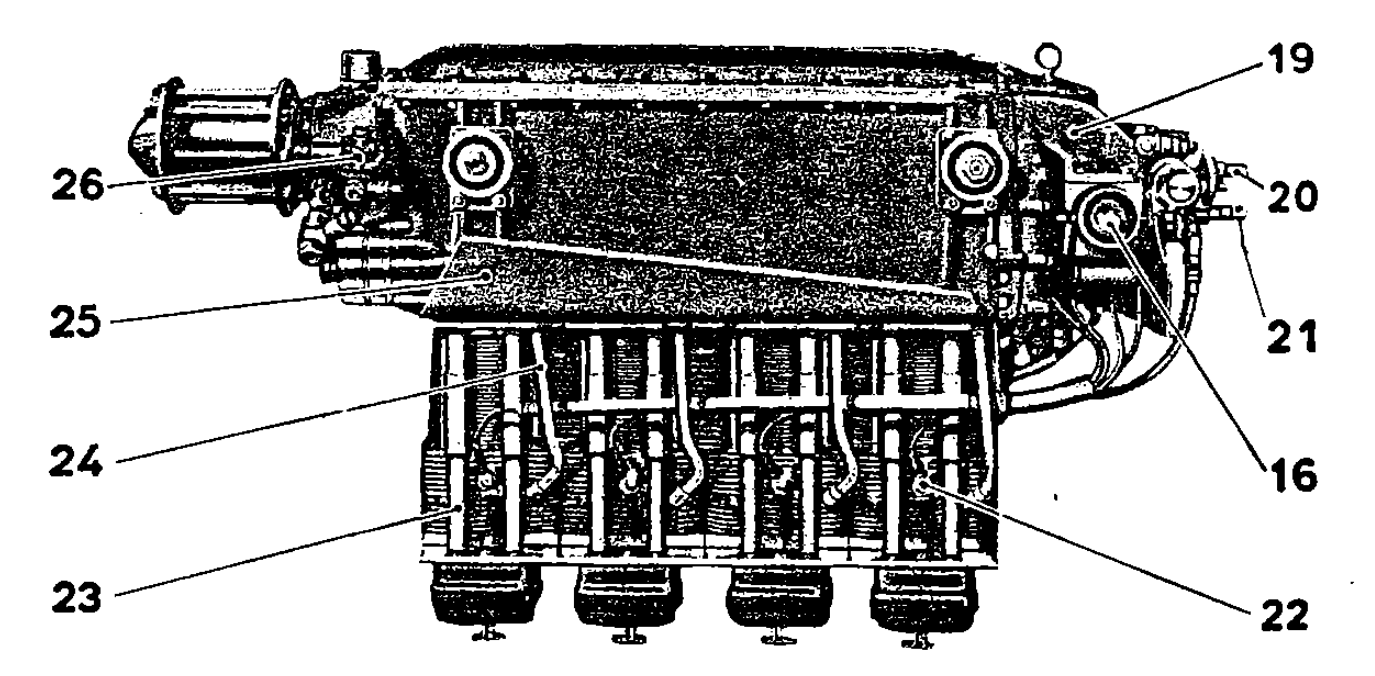
\includegraphics[width=0.95\textwidth]{01-EtudeAeronefs/img/renault4P.png}
  		\legende{Moteur en ligne Renault 4P}{img:renault4P}
	\end{figure}	
 \end{column}
 \end{columns}
 \end{frame}
 
 \begin{frame}{Les principales dispositions de cylindres - moteur en ligne}
	\begin{figure}[H]
  	\scalebox{.3}{\embedvideo*{
\includegraphics[page=1, scale=1]{01-EtudeAeronefs/img/flat4}}{01-EtudeAeronefs/img/video/flat4.mp4}}
  	\legende{Moteur en ligne 4 cylindres}{video:flat4}
	\end{figure}
\end{frame}
 
 \begin{frame}{Les principales dispositions de cylindres - moteur à plat}
 \begin{columns}
 \begin{column}{0.5\textwidth}
 	\begin{itemize}
 		\item Meilleur refroidissement
 		\item Moteur "plat" permettant une meilleure visibilité
 	\end{itemize}
 \end{column}
 \begin{column}{0.5\textwidth}
 	\begin{figure}[H]
  		\centering
    		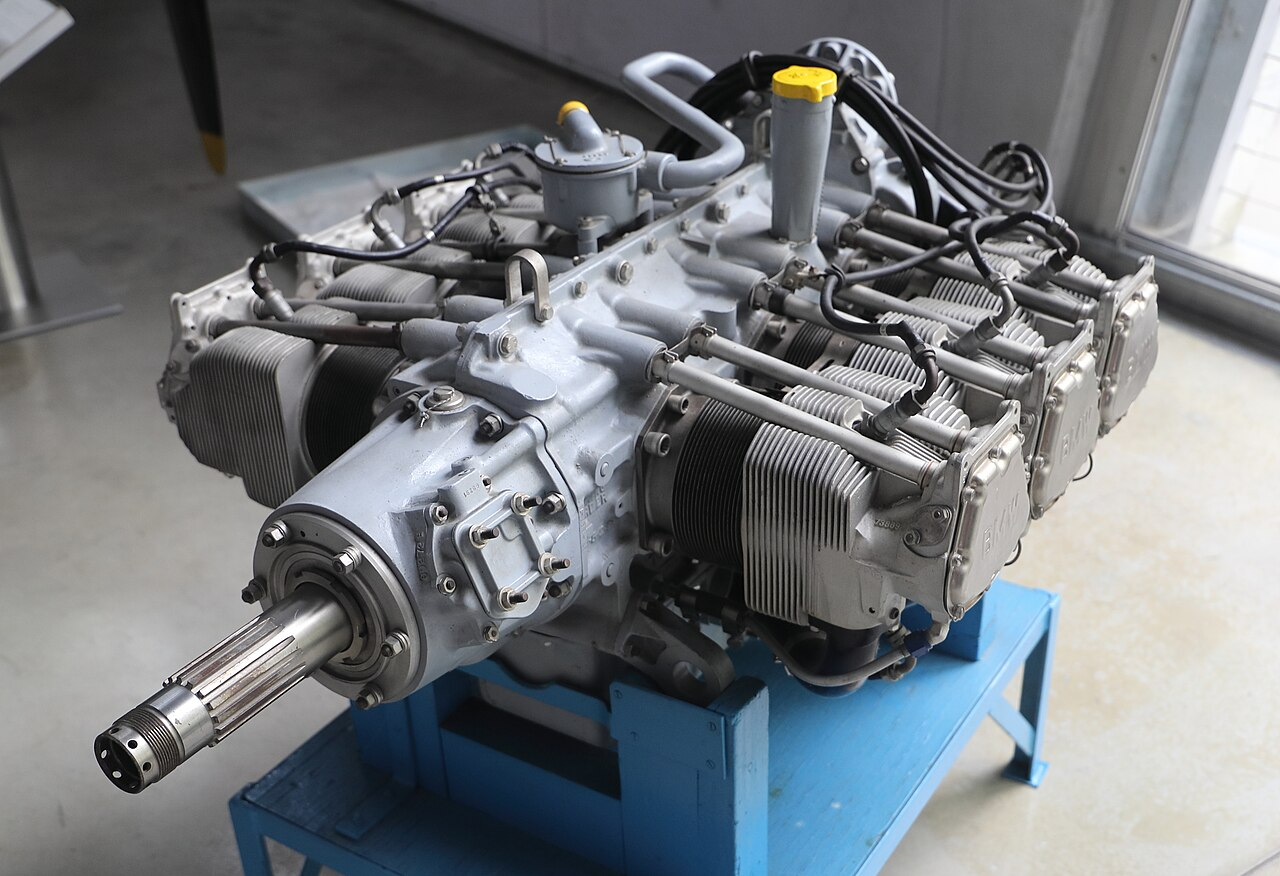
\includegraphics[width=0.95\textwidth]{01-EtudeAeronefs/img/boxer6.jpg}
  		\legende{Moteur à plat 6 cylindres}{img:boxer6}
	\end{figure}	
 \end{column}
 \end{columns}
 \end{frame}

\begin{frame}{Les principales dispositions de cylindres - moteur à plat}
	\begin{figure}[H]
  	\scalebox{.5}{\embedvideo*{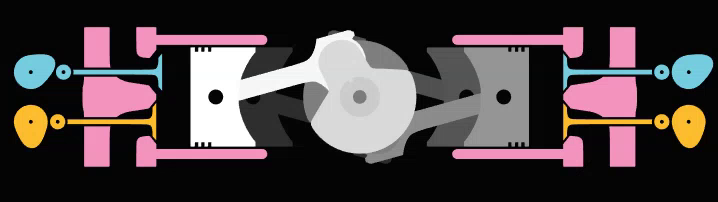
\includegraphics[page=1, scale=1]{01-EtudeAeronefs/img/boxer4}}{01-EtudeAeronefs/img/video/boxer4.mp4}}
  	\legende{Moteur à plat 4 cylindres}{video:boxer4}
	\end{figure}
\end{frame}

\begin{frame}{Les principales dispositions de cylindres - moteur en V}
 \begin{columns}
 \begin{column}{0.5\textwidth}
 	\begin{itemize}
 		\item plus court et plus léger qu'un moteur en ligne équivalent
 		\item Moins de vibrations
 	\end{itemize}
 \end{column}
 \begin{column}{0.5\textwidth}
 	\begin{figure}[H]
  		\centering
    		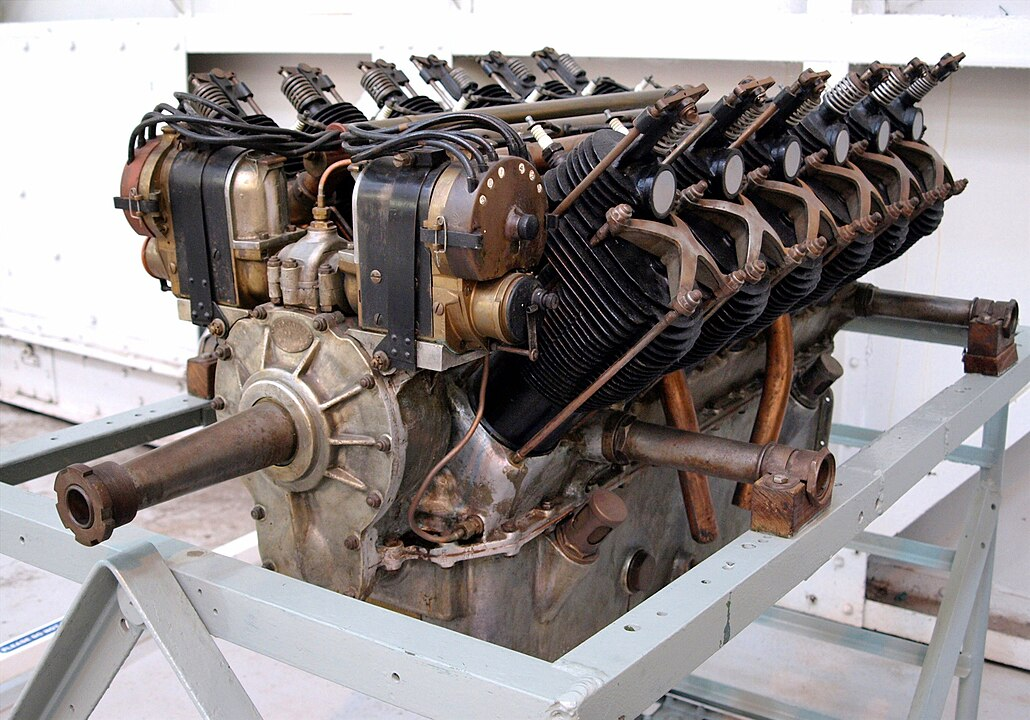
\includegraphics[width=0.95\textwidth]{01-EtudeAeronefs/img/moteurV12.jpg}
  		\legende{Moteur V12}{img:moteurV12}
	\end{figure}	
 \end{column}
 \end{columns}
 \end{frame}
 
 \begin{frame}{Les principales dispositions de cylindres - moteur en V}
	\begin{figure}[H]
  	\scalebox{.32}{\embedvideo*{
\includegraphics[page=1, scale=1]{01-EtudeAeronefs/img/v6}}{01-EtudeAeronefs/img/video/v6.mp4}}
  	\legende{Moteur V6}{video:v6}
	\end{figure}
\end{frame}

\begin{frame}{Les principales dispositions de cylindres - étoile}
 \begin{columns}
 \begin{column}{0.5\textwidth}
 	\begin{itemize}
 		\item Compact, léger, peu coûteux
 		\item Système de graissage adapté au vol acrobatique
 		\item Refroidissement optimum
 	\end{itemize}
 \end{column}
 \begin{column}{0.5\textwidth}
 	\begin{figure}[H]
  		\centering
    		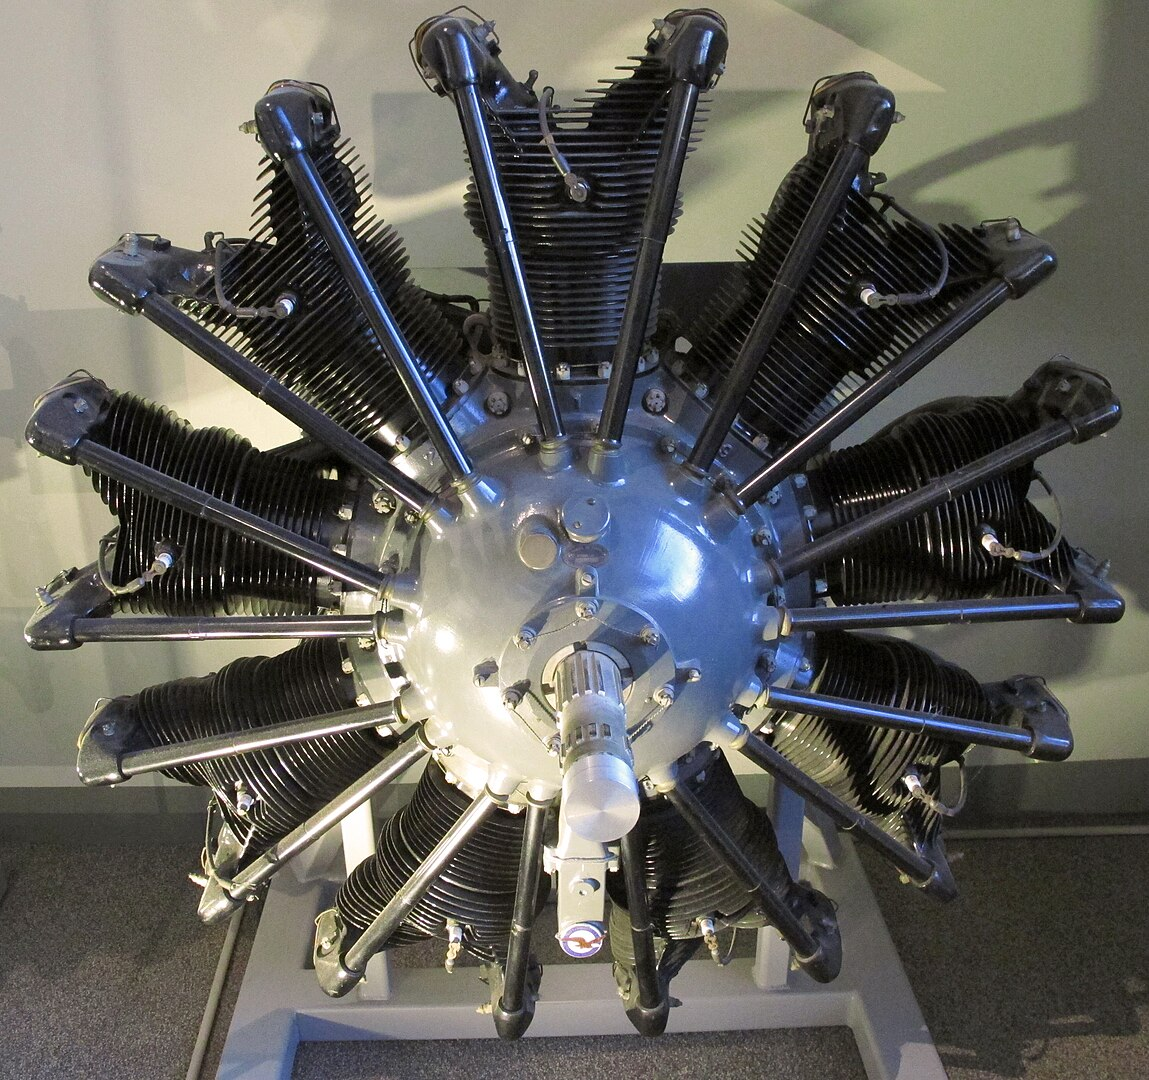
\includegraphics[width=0.95\textwidth]{01-EtudeAeronefs/img/PWWasp.jpg}
  		\legende{Moteur en étoile P\& W Wasp}{img:PWWasp}
	\end{figure}	
 \end{column}
 \end{columns}
 \end{frame}

\begin{frame}{Les principales dispositions de cylindres - étoile}
 \begin{figure}[H]
  	\scalebox{.35}{\embedvideo*{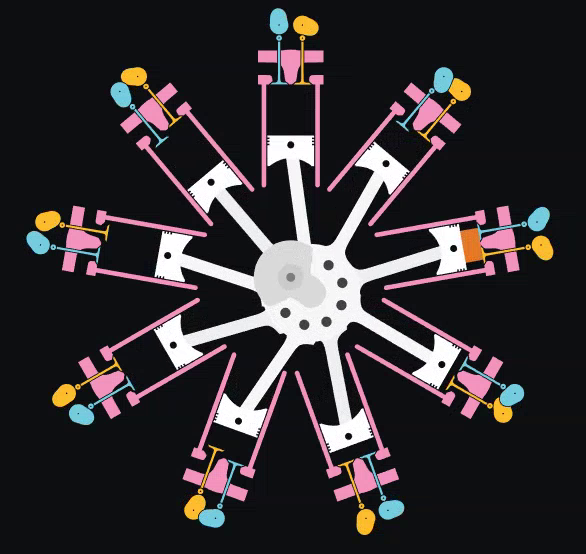
\includegraphics[page=1, scale=1]{01-EtudeAeronefs/img/9cylindresEtoile}}{01-EtudeAeronefs/img/video/9cylindresEtoile.mp4}}
  	\legende{Moteur en étoile 9 cylindres}{video:9CylindresEtoile}
	\end{figure}
	\end{frame}
	
\section{Turbomoteurs}
 \subsection{Réacteurs}
 \begin{frame}{Turboréacteur simple flux \anglais{Turbojet}}
 	\begin{figure}[H]
  		\centering
    		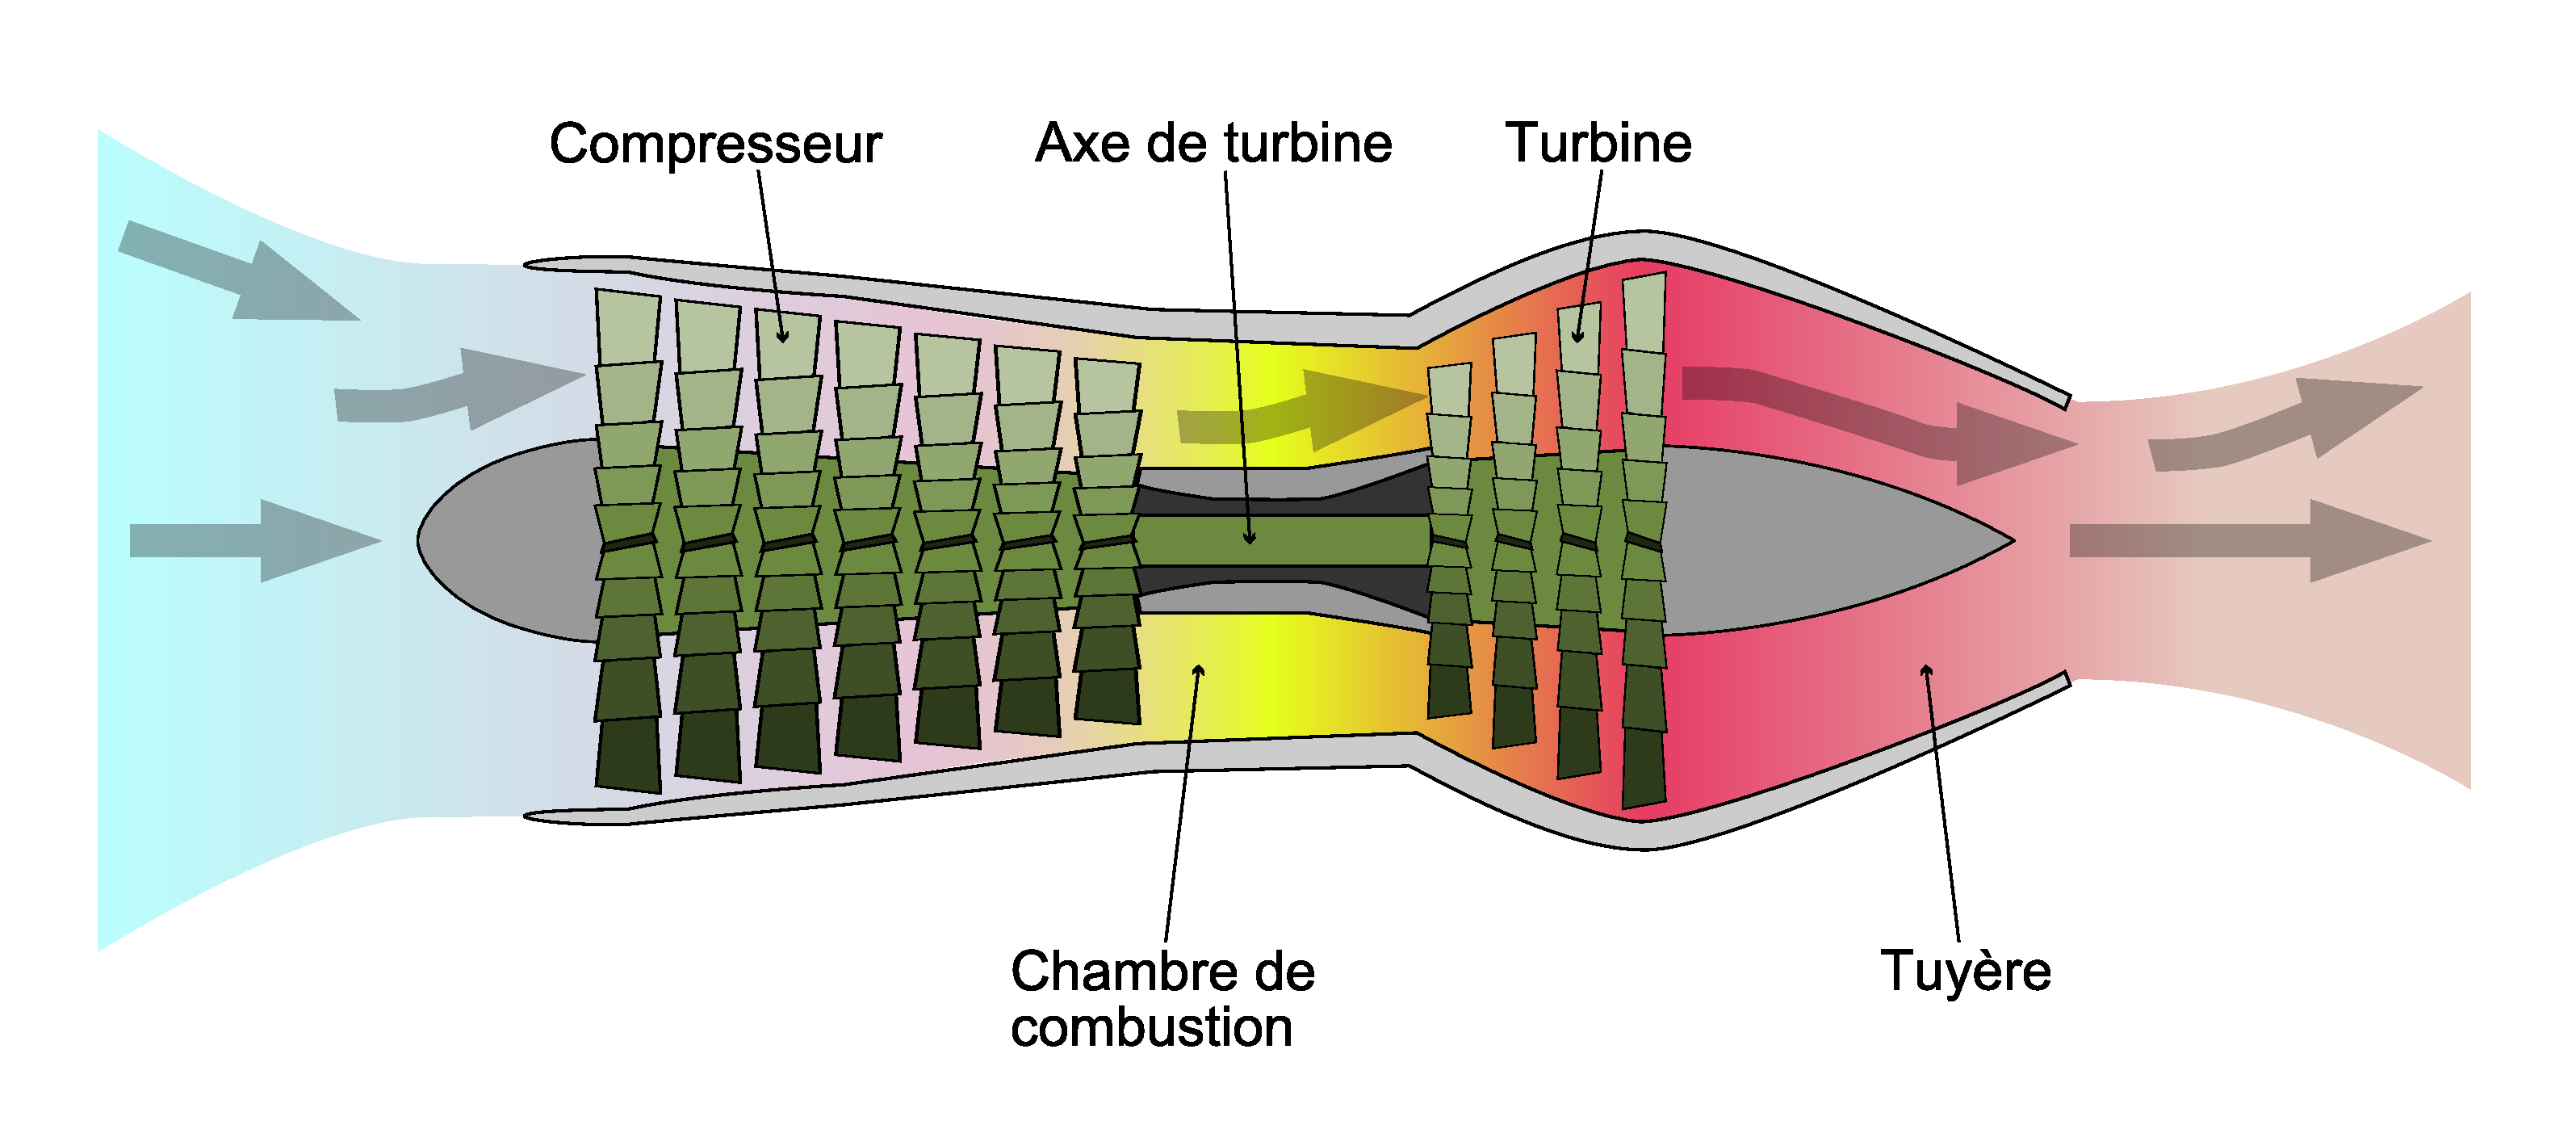
\includegraphics[width=1.0\textwidth]{01-EtudeAeronefs/img/turbomachines/turboreacteur-simpleFlux.pdf}
  		\legende{Schéma d'un turboréacteur simple corps simple flux}{img:turboreacteur-simpleFlux}
	\end{figure}	
  \end{frame}
  
  \begin{frame}{Turboréacteurs - avantages}
  	Depuis sa mise au point des turboréacteurs à la fin des années 1930, le réacteur s'est peu à peu imposé sur de très nombreux avions. C'est en effet un motorisation qui présente de nombreux avantages :
  	\begin{itemize}
  			\item Puissance
  			\item Légèreté comparé à des moteurs à explosion et hélices de même puissance
  			\item Très fiable (mouvement purement rotatif), engendre moins de vibrations
  			\item Permet d'atteindre les très hautes vitesses
  	\end{itemize}
  	
  	\begin{columns}
  	\begin{column}{0.5\textwidth}
  	\begin{figure}[H]
  		\centering
    		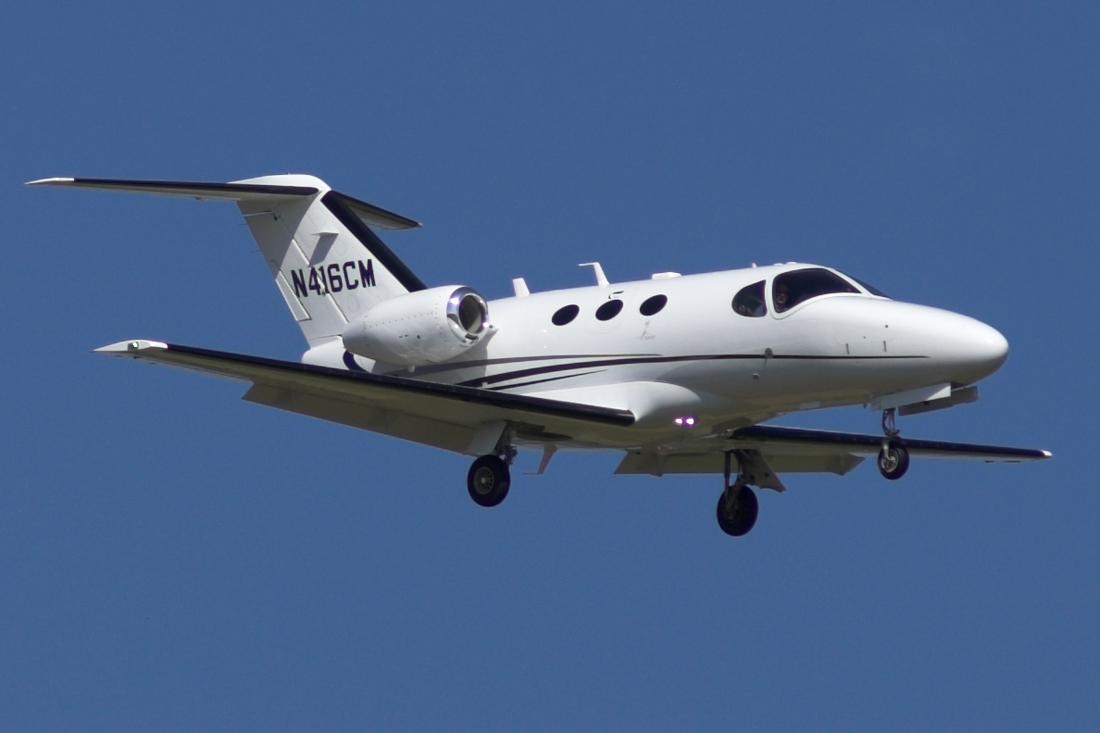
\includegraphics[width=0.4\textwidth]{01-EtudeAeronefs/img/Cessna_Citation_Mustang.jpg}
  		\legende{Cessna Citation Mustang équipé de réacteurs P\&W PW615, 140 kg, puissance jusqu'à 1500 CV}{img:Cessna_Citation_Mustang}
	\end{figure}	
  	\end{column}
  	\begin{column}{0.5\textwidth}
  	\begin{figure}[H]
  		\centering
    		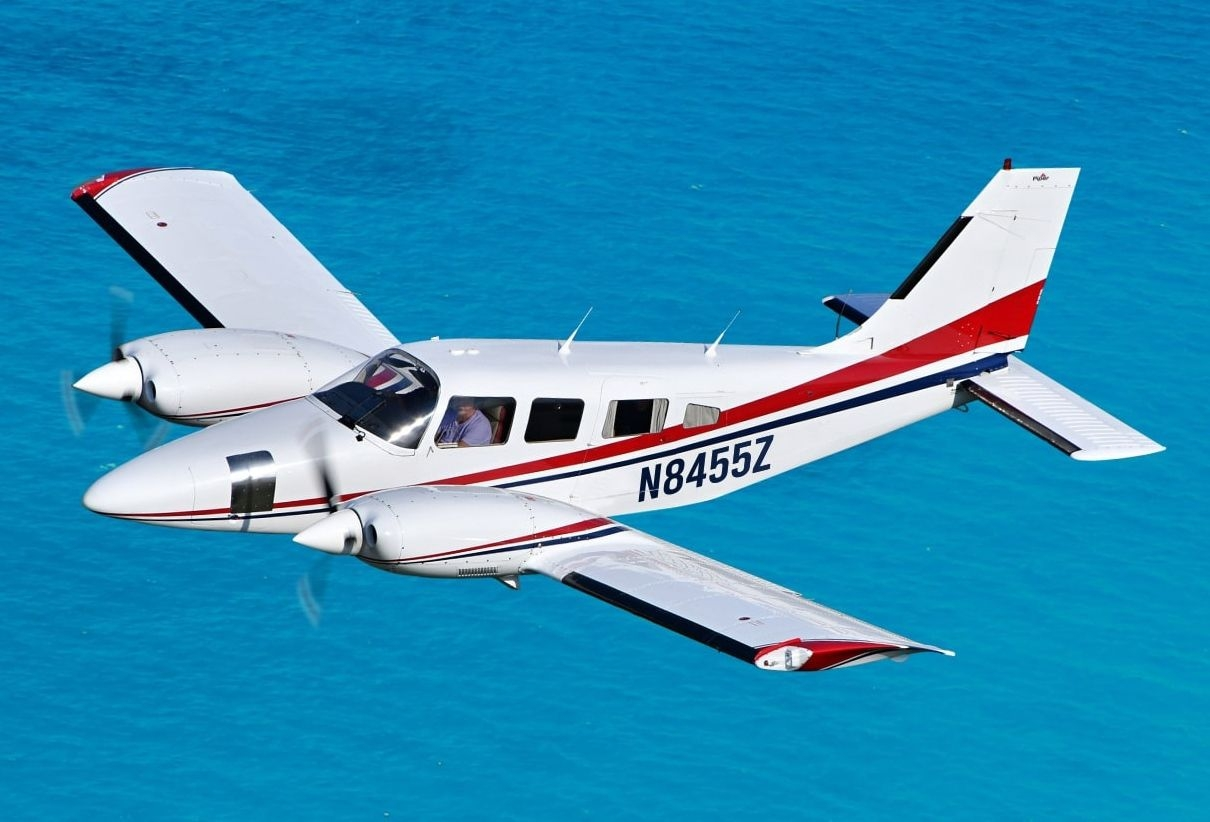
\includegraphics[width=0.4\textwidth]{01-EtudeAeronefs/img/Piper_PA-34.jpg}
  		\legende{Piper PA-34 équipé de moteurs à explosion Lycoming IO-360-C1E6, 139 kg, puissance 200 CV}{img:Piper_PA-34}
	\end{figure}	
  	\end{column}
  	\end{columns}
  \end{frame}
  
  \begin{frame}{Augmenter l'efficacité : le turboréacteur double corps}
	\begin{figure}[H]
  		\centering
    		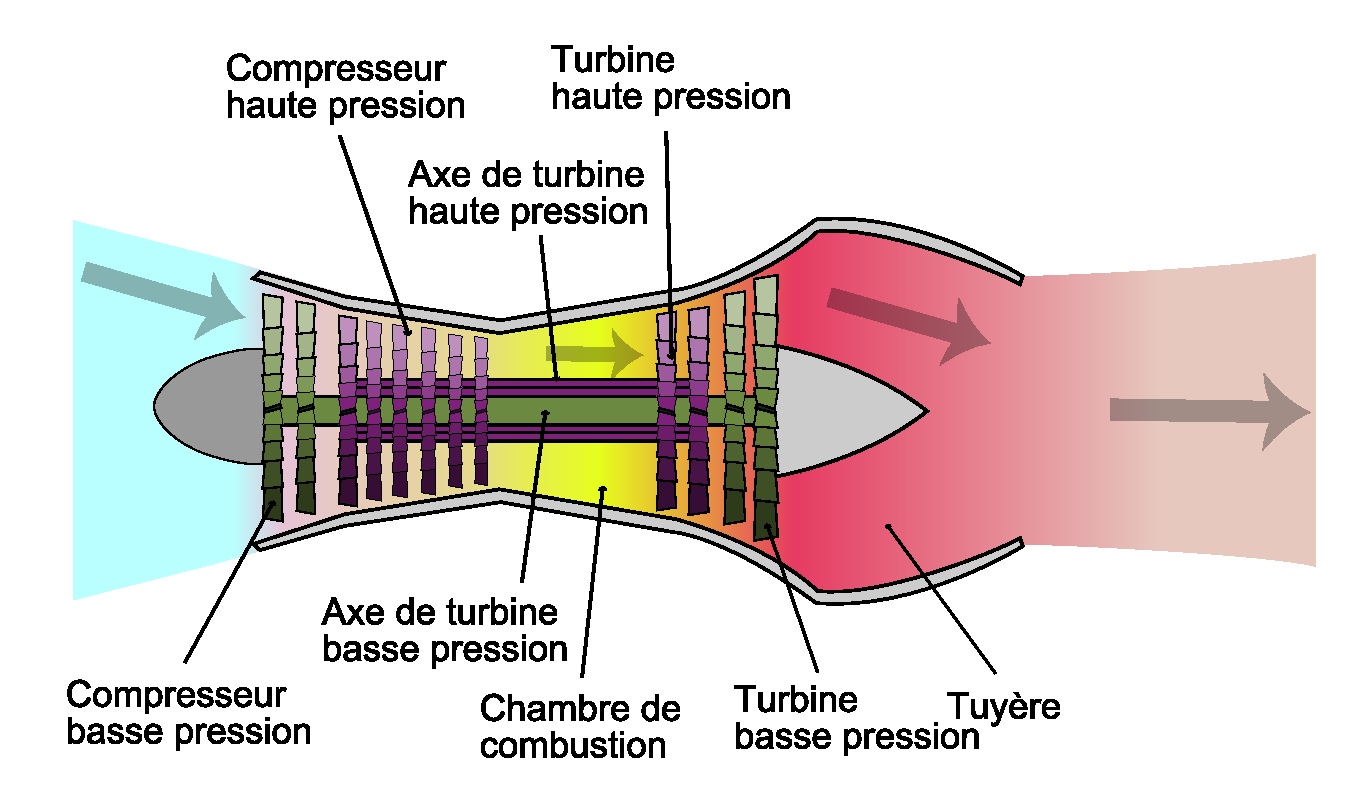
\includegraphics[width=0.8\textwidth]{01-EtudeAeronefs/img/turbomachines/turboreacteur-simpleFluxDoubleCorps.pdf}
  		\legende{Schéma d'un turboréacteur double corps}{img:turboreacteur-simpleFluxDoubleCorps}
		\end{figure}	
 \end{frame}
 
 \begin{frame}{Augmenter l'efficacité : le turboréacteur double corps}
	Comparaison d'un réacteur simple corps avec un réacteur double corps. 
 
 	\begin{columns}
		\begin{column}{0.5\textwidth}
		\begin{figure}[H]
  		\centering
    		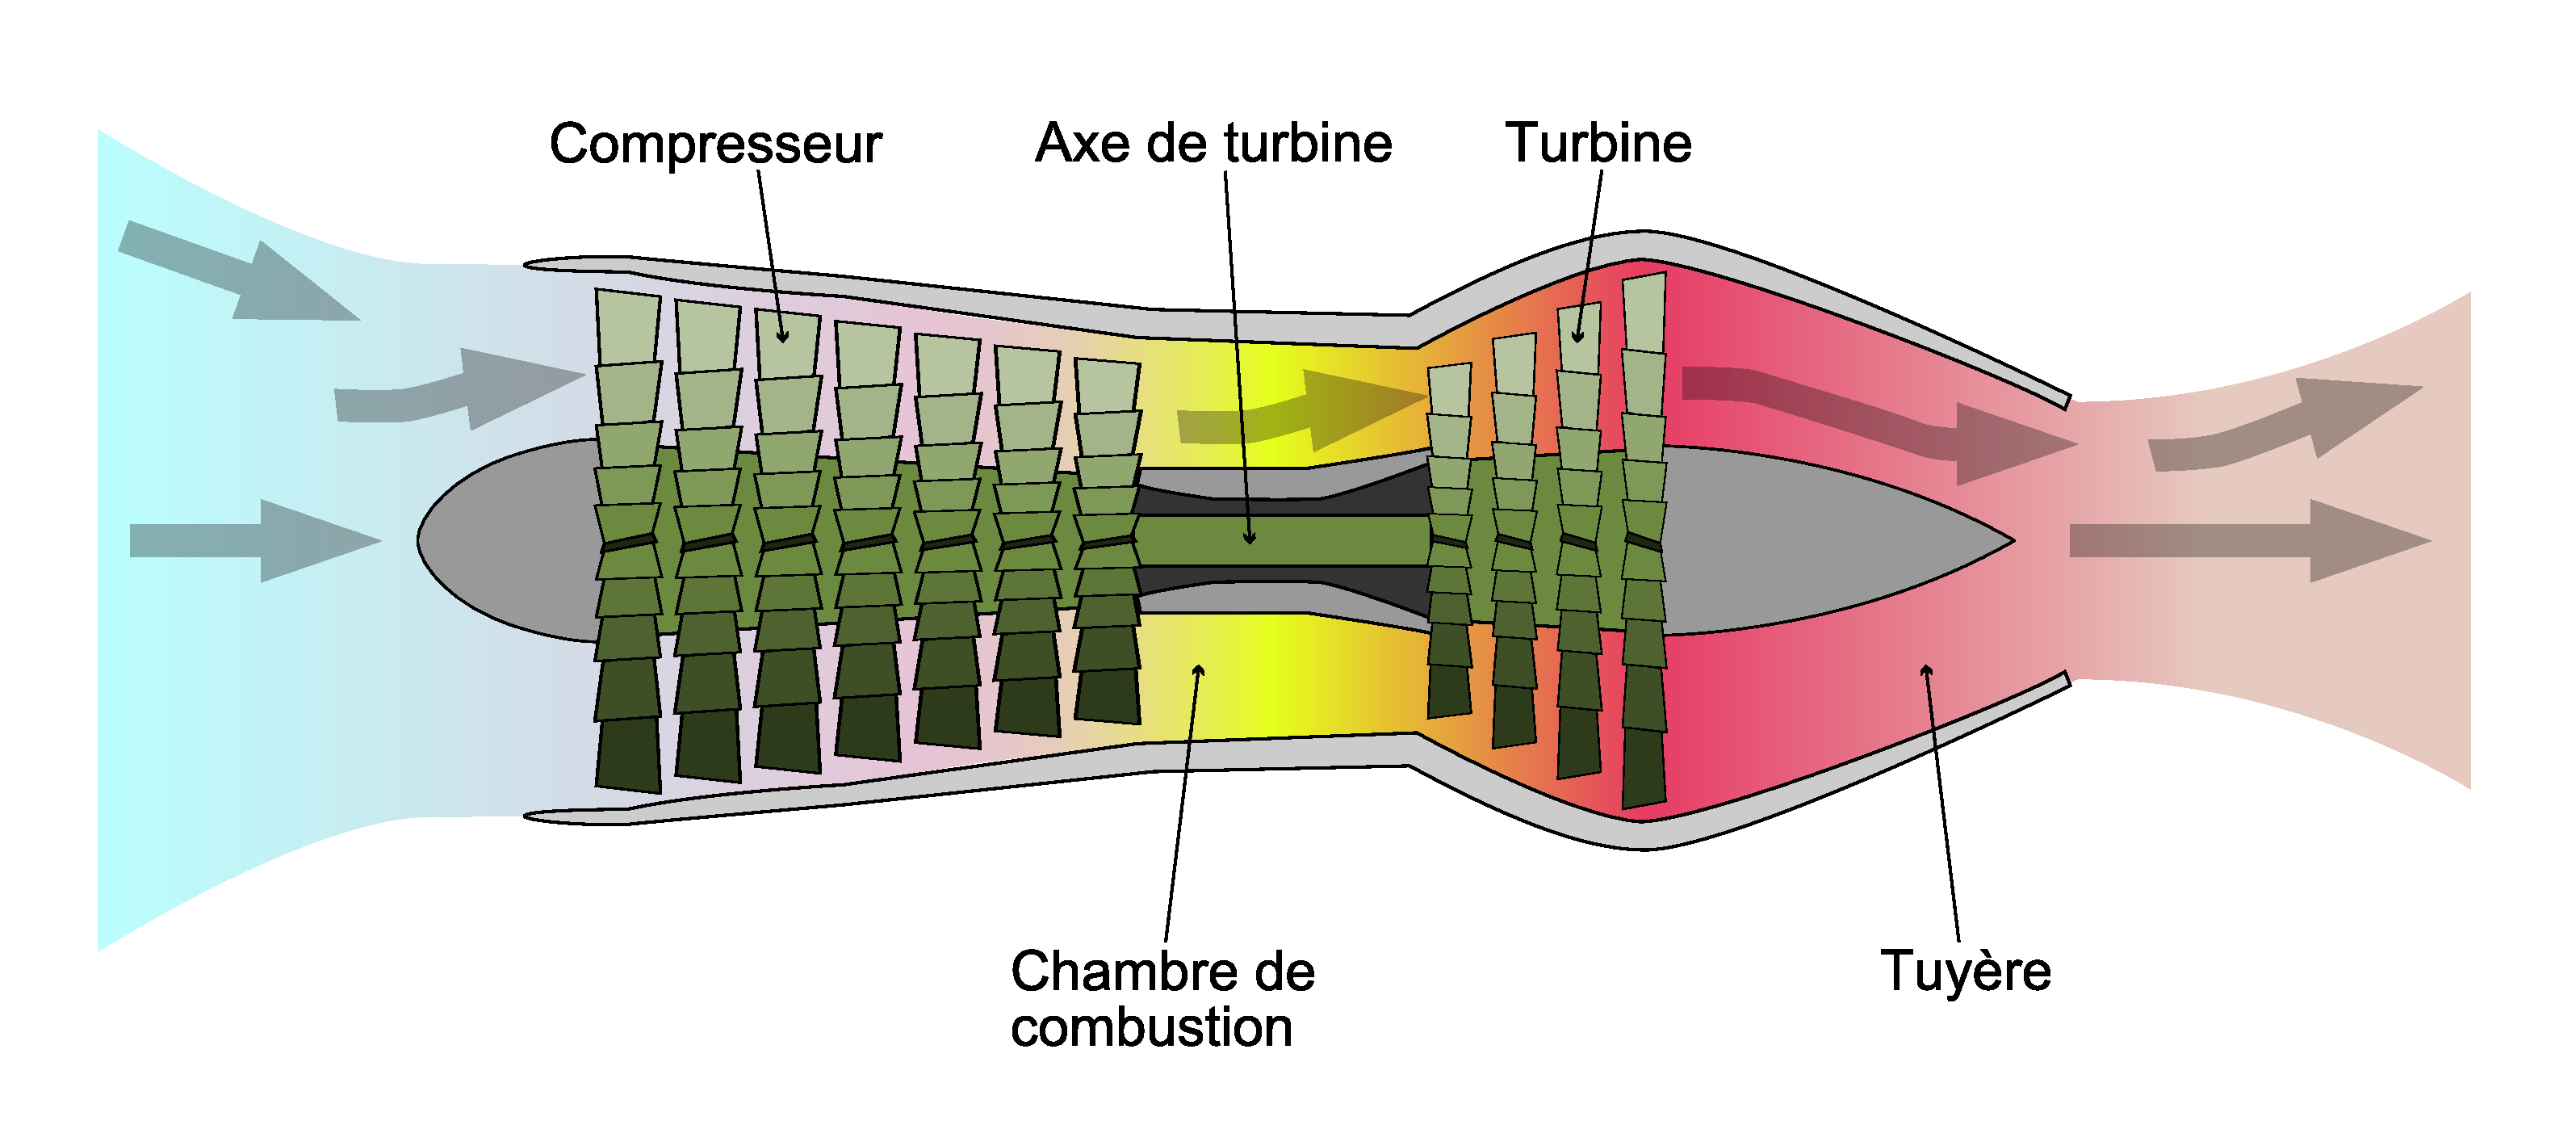
\includegraphics[width=1.1\textwidth]{01-EtudeAeronefs/img/turbomachines/turboreacteur-simpleFlux.pdf}
  		\legende{Schéma d'un turboréacteur simple corps simple flux}{img:turboreacteur-simpleFlux}
	\end{figure}	
	\end{column}
	\begin{column}{0.5\textwidth}
	\begin{figure}[H]
  		\centering
    		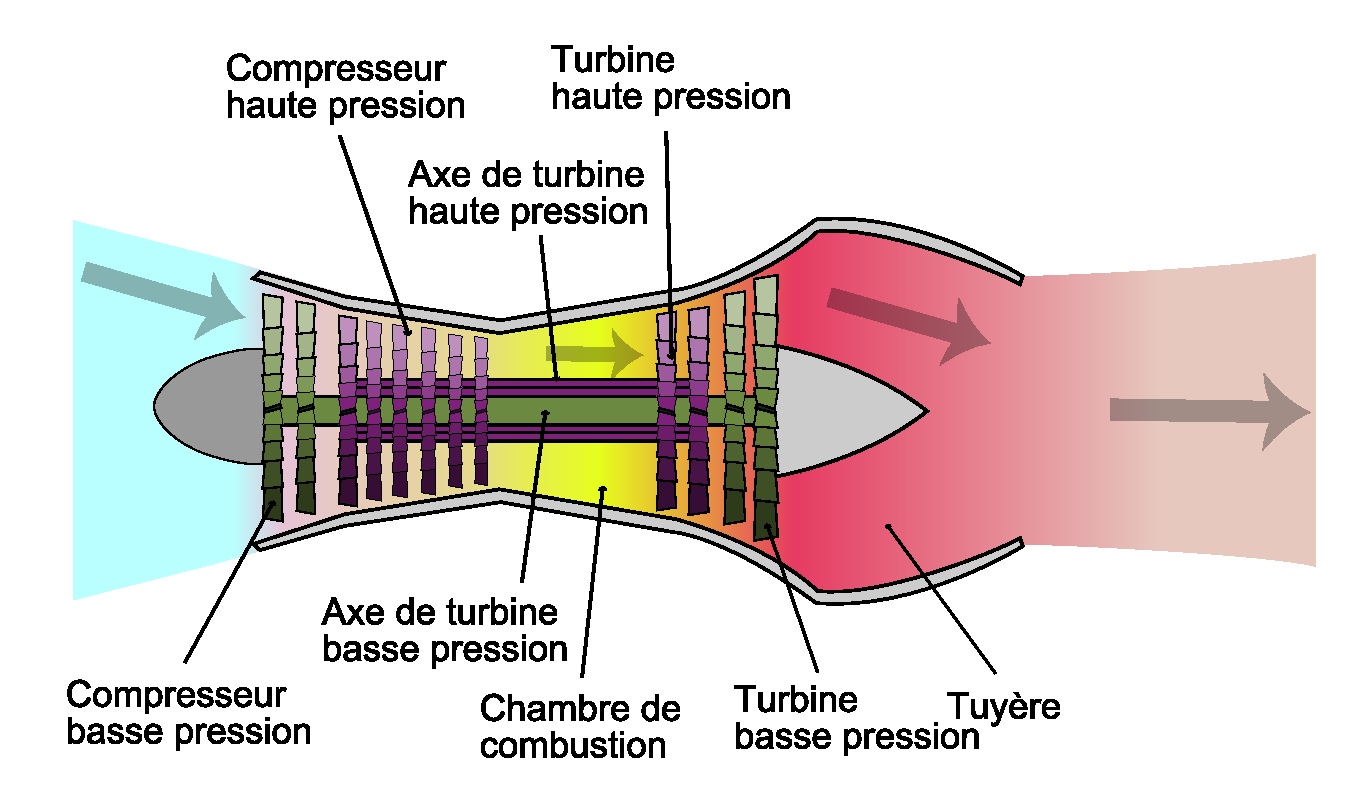
\includegraphics[width=1.1\textwidth]{01-EtudeAeronefs/img/turbomachines/turboreacteur-simpleFluxDoubleCorps.pdf}
  		\legende{Schéma d'un turboréacteur double corps}{img:turboreacteur-simpleFluxDoubleCorps}
		\end{figure}	
		\end{column}
	\end{columns}
 \end{frame}
  
  \begin{frame}{Turboréacteur double flux \anglais{Turbofan}}
	\begin{figure}[H]
  		\centering
    		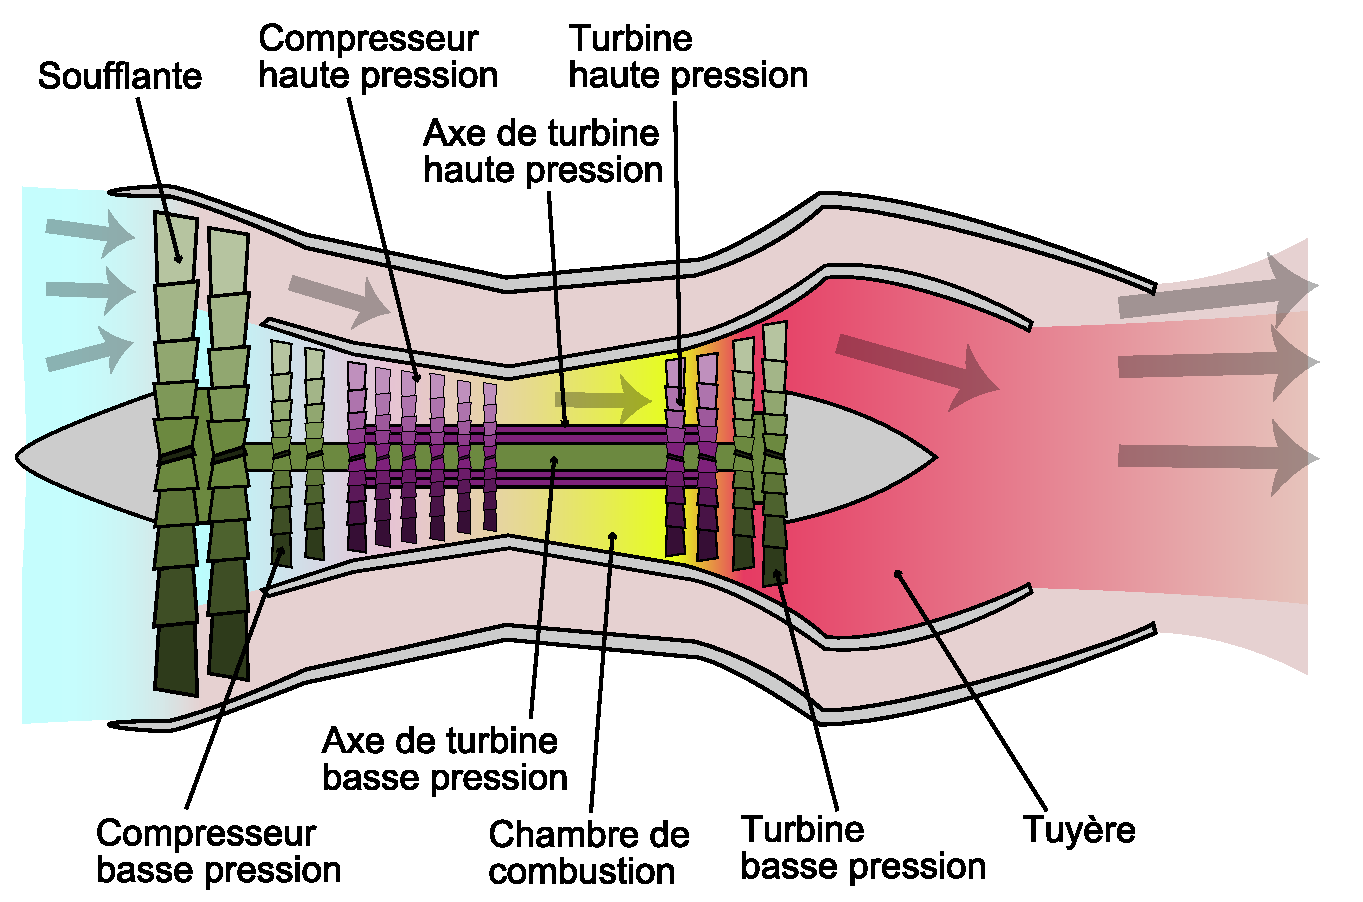
\includegraphics[width=0.7\textwidth]{01-EtudeAeronefs/img/turbomachines/turboreacteur-doubleFlux.pdf}
  		\legende{Schéma d'un turboréacteur double corps double flux}{img:turboreacteur-doubleFlux}
		\end{figure}	
 \end{frame}
 
  \begin{frame}{Turboréacteur double flux \anglais{Turbofan}}
 	\begin{columns}
 	\begin{column}{0.5\textwidth}
		\begin{figure}[H]
  		\centering
    		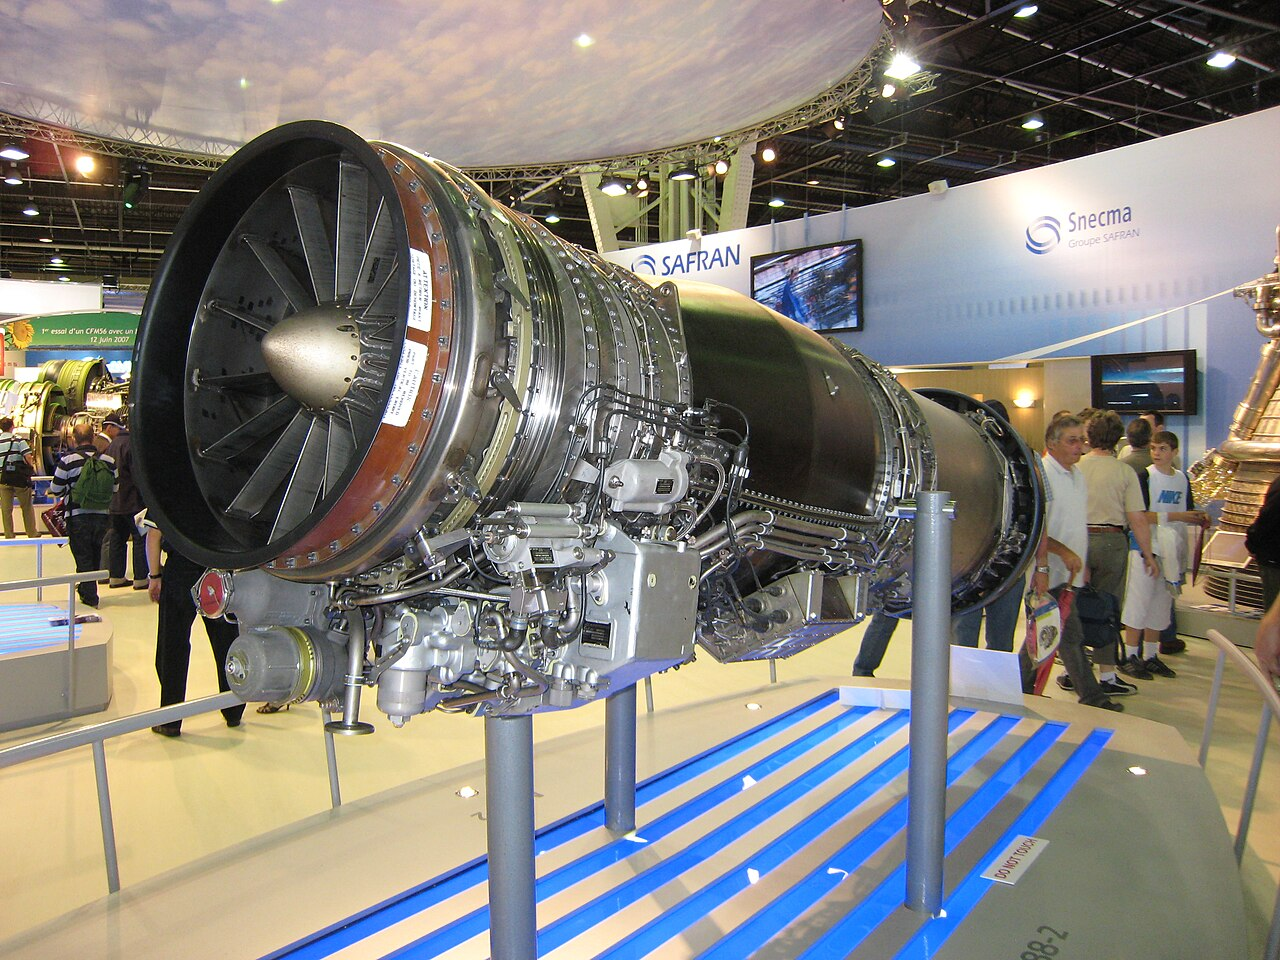
\includegraphics[width=0.96\textwidth]{01-EtudeAeronefs/img/M88}
  		\legende{Réacteur double flux militaire : M88 du Rafale, 900 kg, 5/7.5 tonnes de poussée}{img:M88}
		\end{figure}	
   \end{column}
   \begin{column}{0.5\textwidth}
		\begin{figure}[H]
  		\centering
    		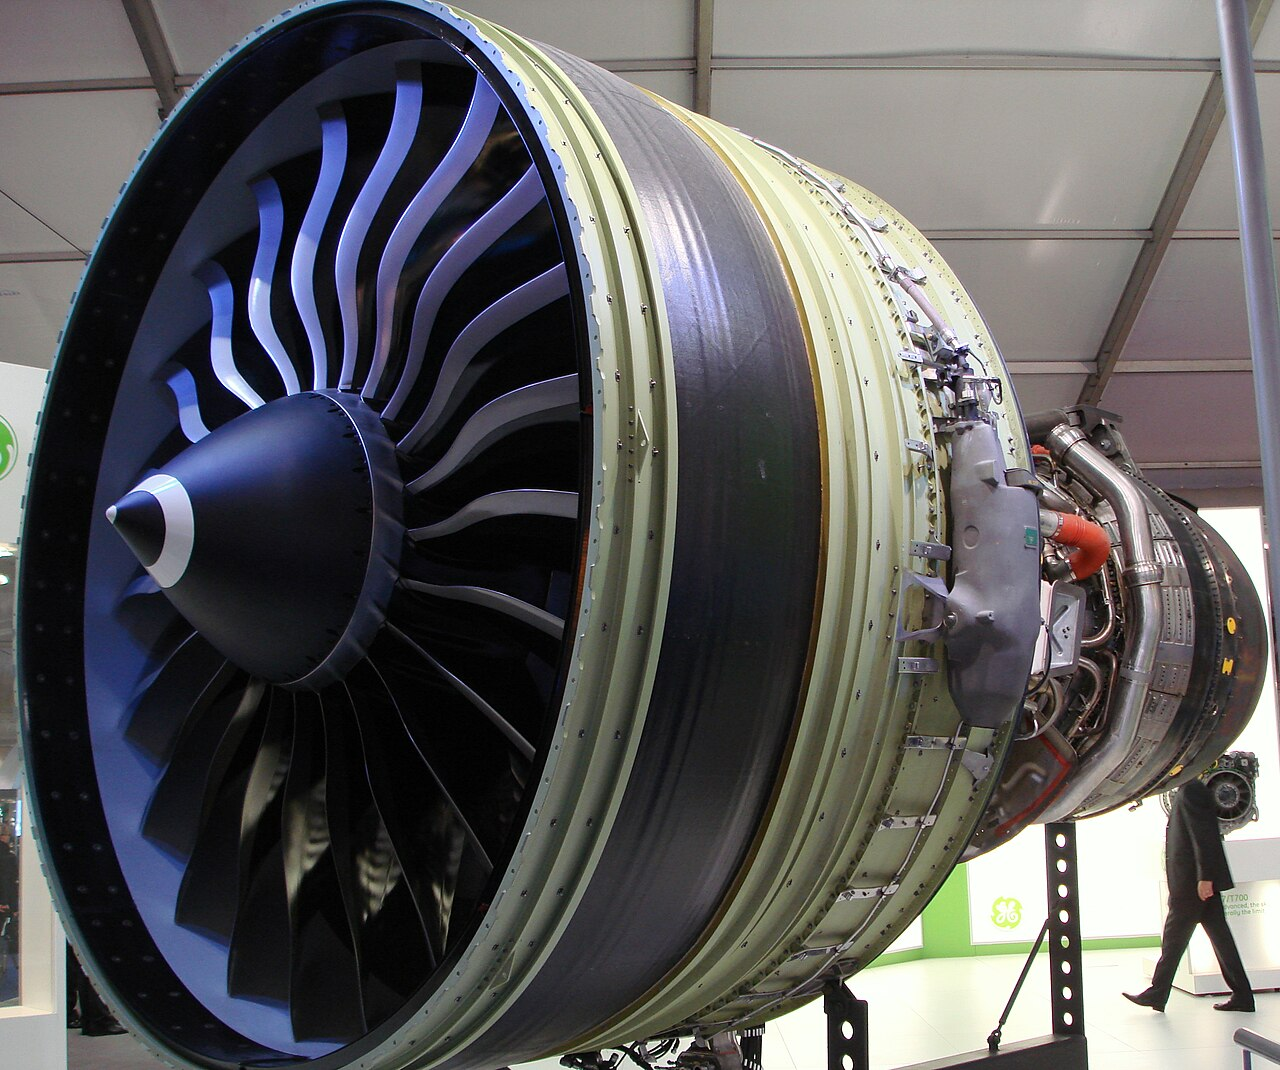
\includegraphics[width=0.95\textwidth]{01-EtudeAeronefs/img/GE90}
  		\legende{Réacteur double flux civil : GE90 du Boeing 777, 3,43~m de diamètre, 8,3~tonnes, 57 tonnes de poussée, 110~000~CV}{img:GE90}
		\end{figure}
   \end{column}
 	\end{columns}
	
 \end{frame}
 
 \begin{frame}{Turboréacteur double flux \anglais{Turbofan} - Avantages}
 	\begin{columns}
 	\begin{column}{0.35\textwidth}
		\begin{figure}[H]
  		\centering
    		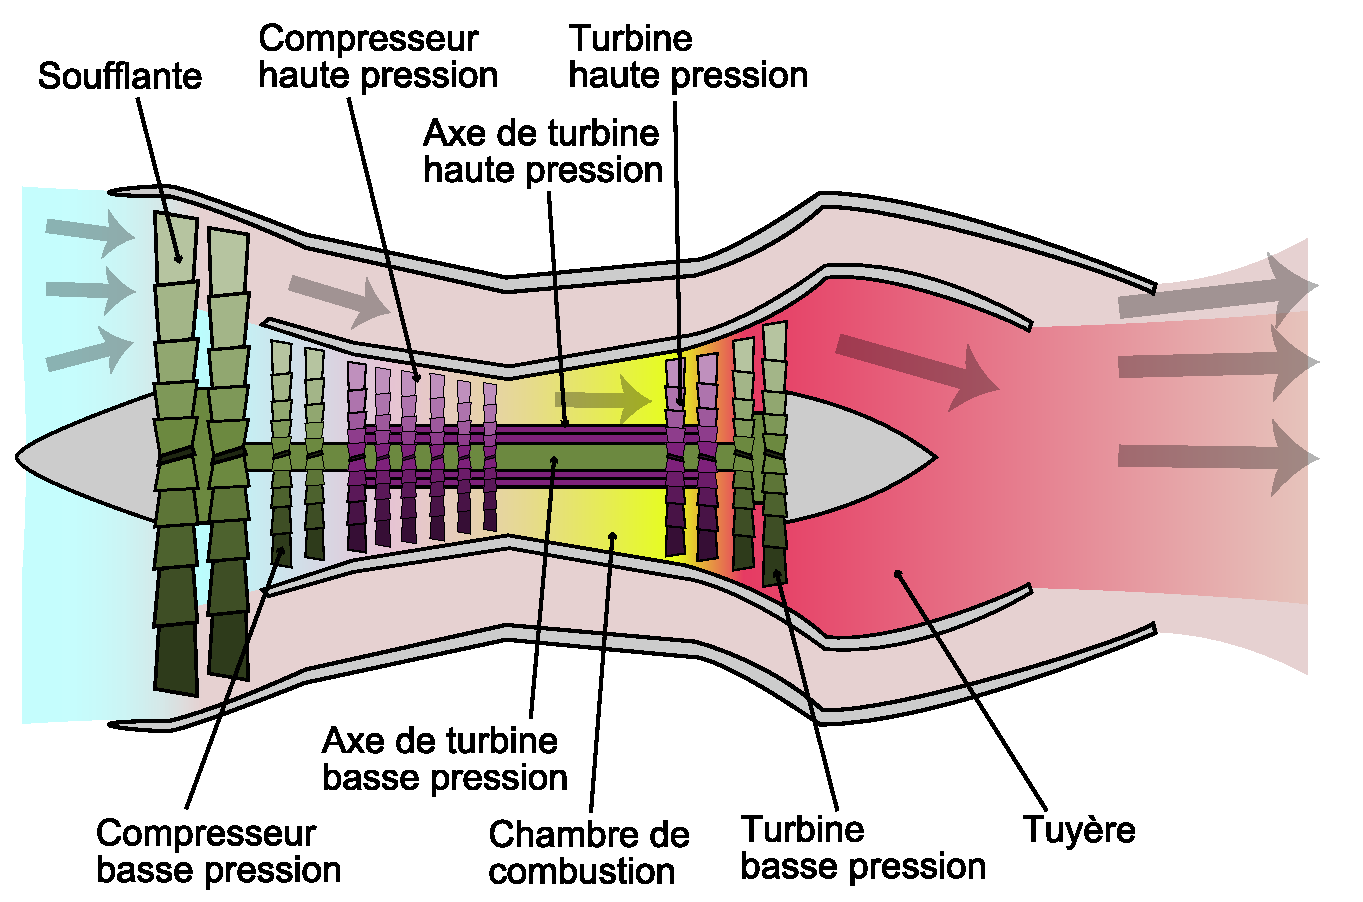
\includegraphics[width=1.24\textwidth]{01-EtudeAeronefs/img/turbomachines/turboreacteur-doubleFlux.pdf}
  		\legende{}{img:turboreacteur-doubleFlux}
		\end{figure}	
   \end{column}
   \begin{column}{0.65\textwidth}
		\begin{itemize}
			\item Jusqu'à 80\% de la poussée assurée par la soufflante
			\item Plus silencieux qu'un simple flux
			\item Plus économique : moins de consommation de carburant, c'est aussi moins de $CO_2$
			\item Taux de dilution : rapport entre le volume d'air du flux primaire et du flux secondaire : 
			\begin{itemize}
				\item Faible taux de dilution (moins de 1) : usage militaire (0.3 pour le M88)
				\item Taux de dilution moyen : jets d'affaire
				\item Fort taux de dilution (au dessus de 5) : avions de ligne (9 pour le GE90) 	
			\end{itemize}			 
		\end{itemize}
   \end{column}
 	\end{columns}
	
 \end{frame}
  
  \begin{frame}{Post-combustion \anglais{afterburner} - Principe}
	\begin{figure}[H]
  		\centering
    		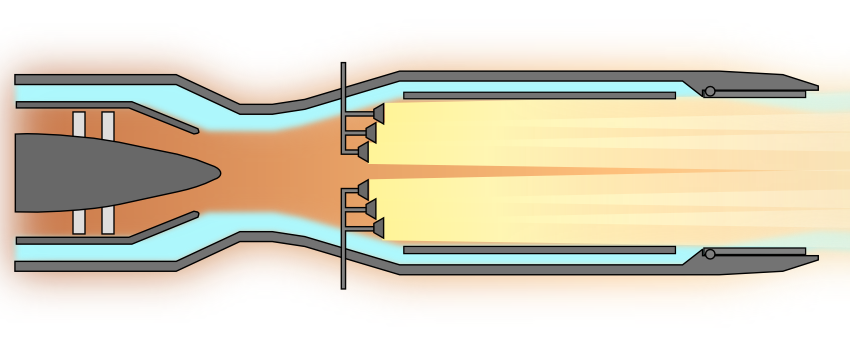
\includegraphics[width=0.7\textwidth]{01-EtudeAeronefs/img/postcombustion.png}
  		\legende{Une post-combustion}{img:postcombustion}
	\end{figure}	
	\begin{columns}
	\begin{column}{0.5\textwidth}
		\begin{itemize}
			\item Injection de carburant en sortie de tuyère
		\end{itemize}
	\end{column}
 	\begin{column}{0.5\textwidth}
		\begin{itemize}
			\pause
			\item Augmentation de la poussée
			\pause
			\item Très bruyant
			\item Très forte consommation
		\end{itemize}
   \end{column}
   \end{columns}	
  \end{frame}
  \begin{frame}{Post-combustion \anglais{afterburner}}
	\begin{figure}[H]
  		\centering 
    		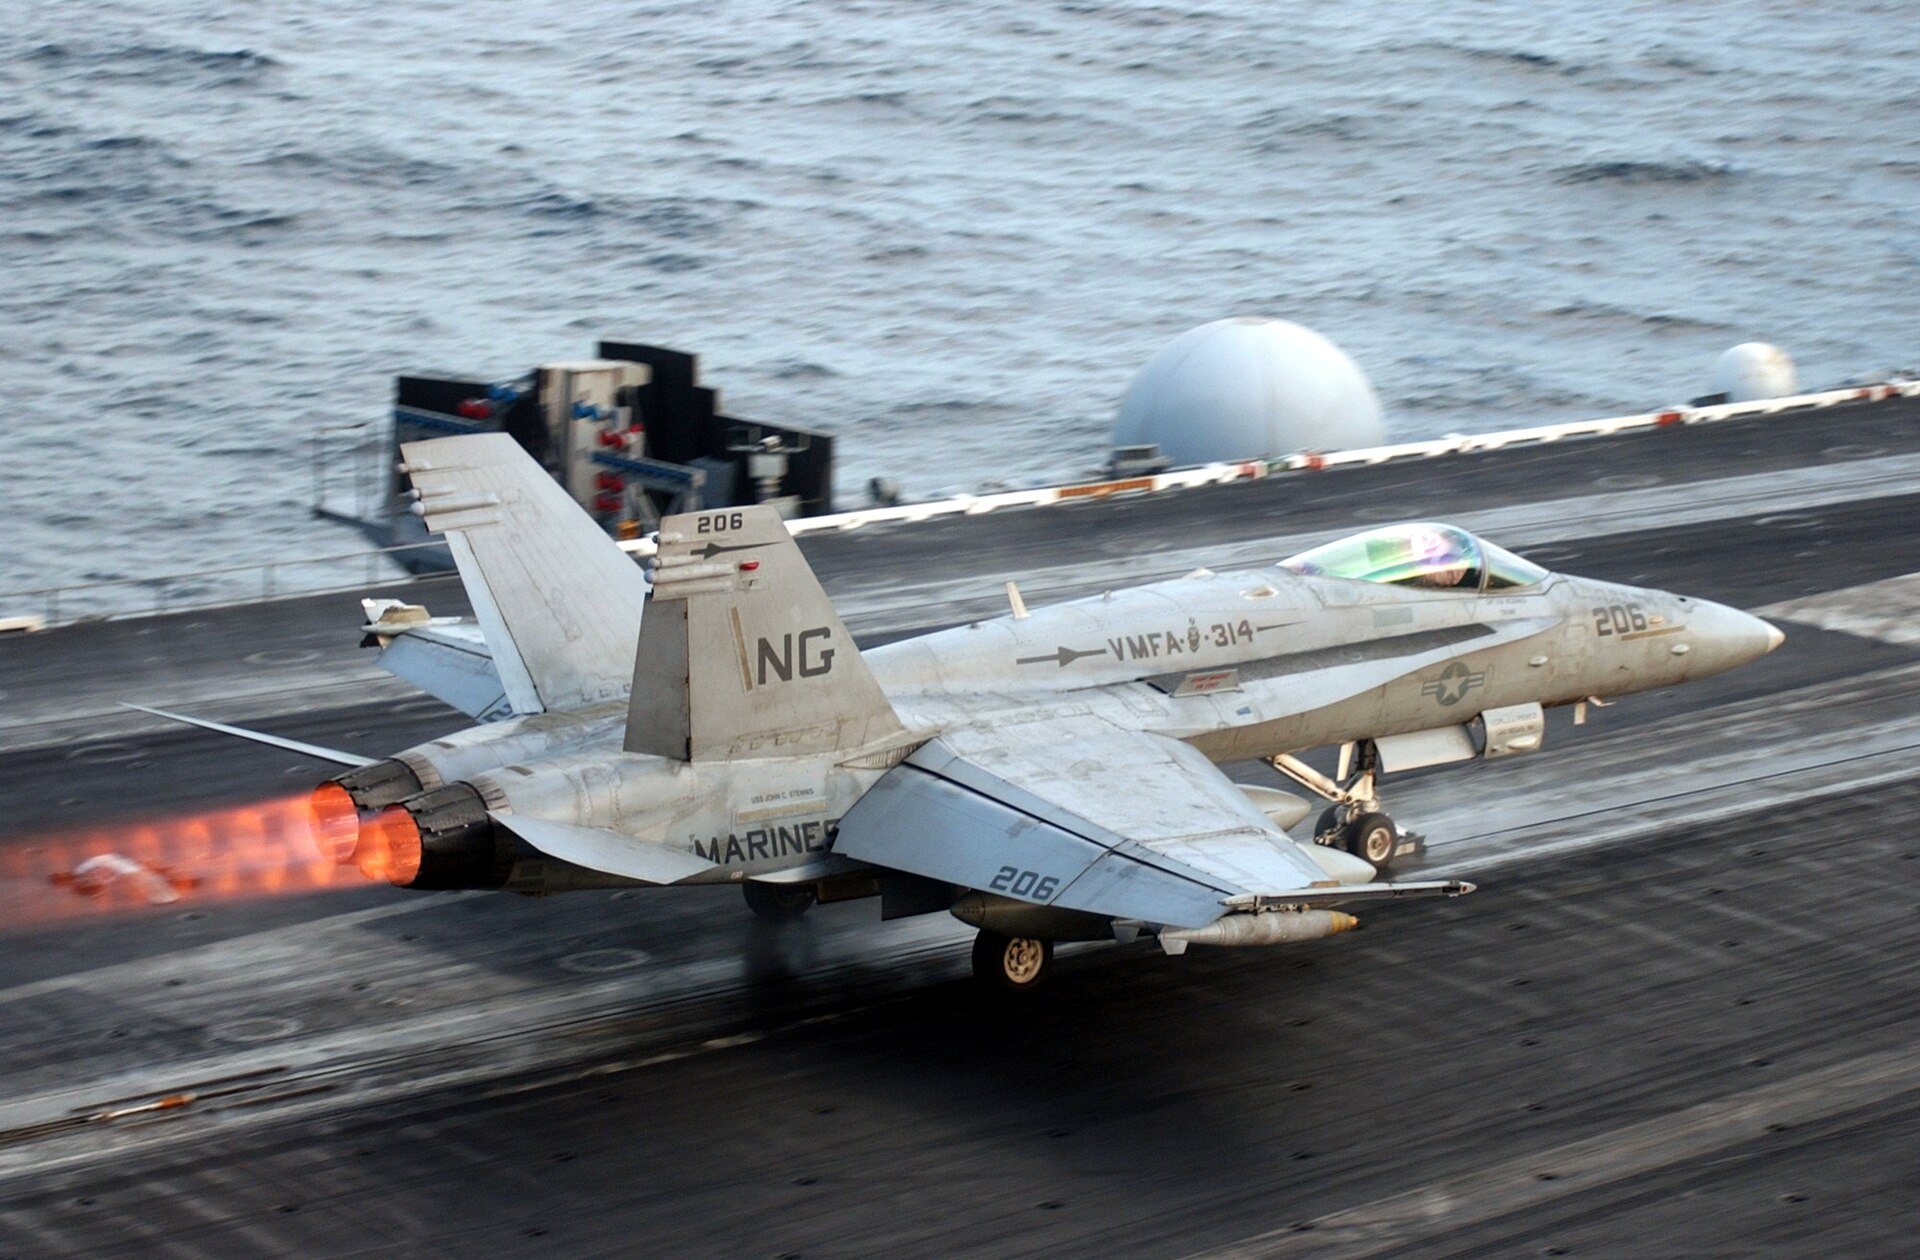
\includegraphics[width=0.3\textwidth]{01-EtudeAeronefs/img/postcombustion-FA-18.jpg}
  		\legende{F18 au décollage avec PC}{img:postcombustion-FA-18}
	\end{figure}	
	\begin{table}[]
\begin{tabular}{l|l|l|}
\cline{2-3}
                                            & Concorde          & Rafale              \\ \hline
\multicolumn{1}{|l|}{Moteur}                & 4 Olympus 593     & 2 M88               \\ \hline
\multicolumn{1}{|l|}{Consommation avec PC}  & 80 t/h            & 20 t/h              \\ \hline
\multicolumn{1}{|l|}{Consommation à "sec"}  & 20 t/h            & 2.5 t/h             \\ \hline
\multicolumn{1}{|l|}{Capacité en carburant} & 100 t             & 11,5 t              \\ \hline
\multicolumn{1}{|l|}{Poussée à sec/avec PC} & 56 t/68 t (+22\%) & 100 t/150 t (+25\%) \\ \hline
\end{tabular}
\end{table}		
  \end{frame}
 
 
 \subsection{Turbopropulseurs} 
   \begin{frame}{Turbopropulseur}
	\begin{figure}[H]
  	\centering
    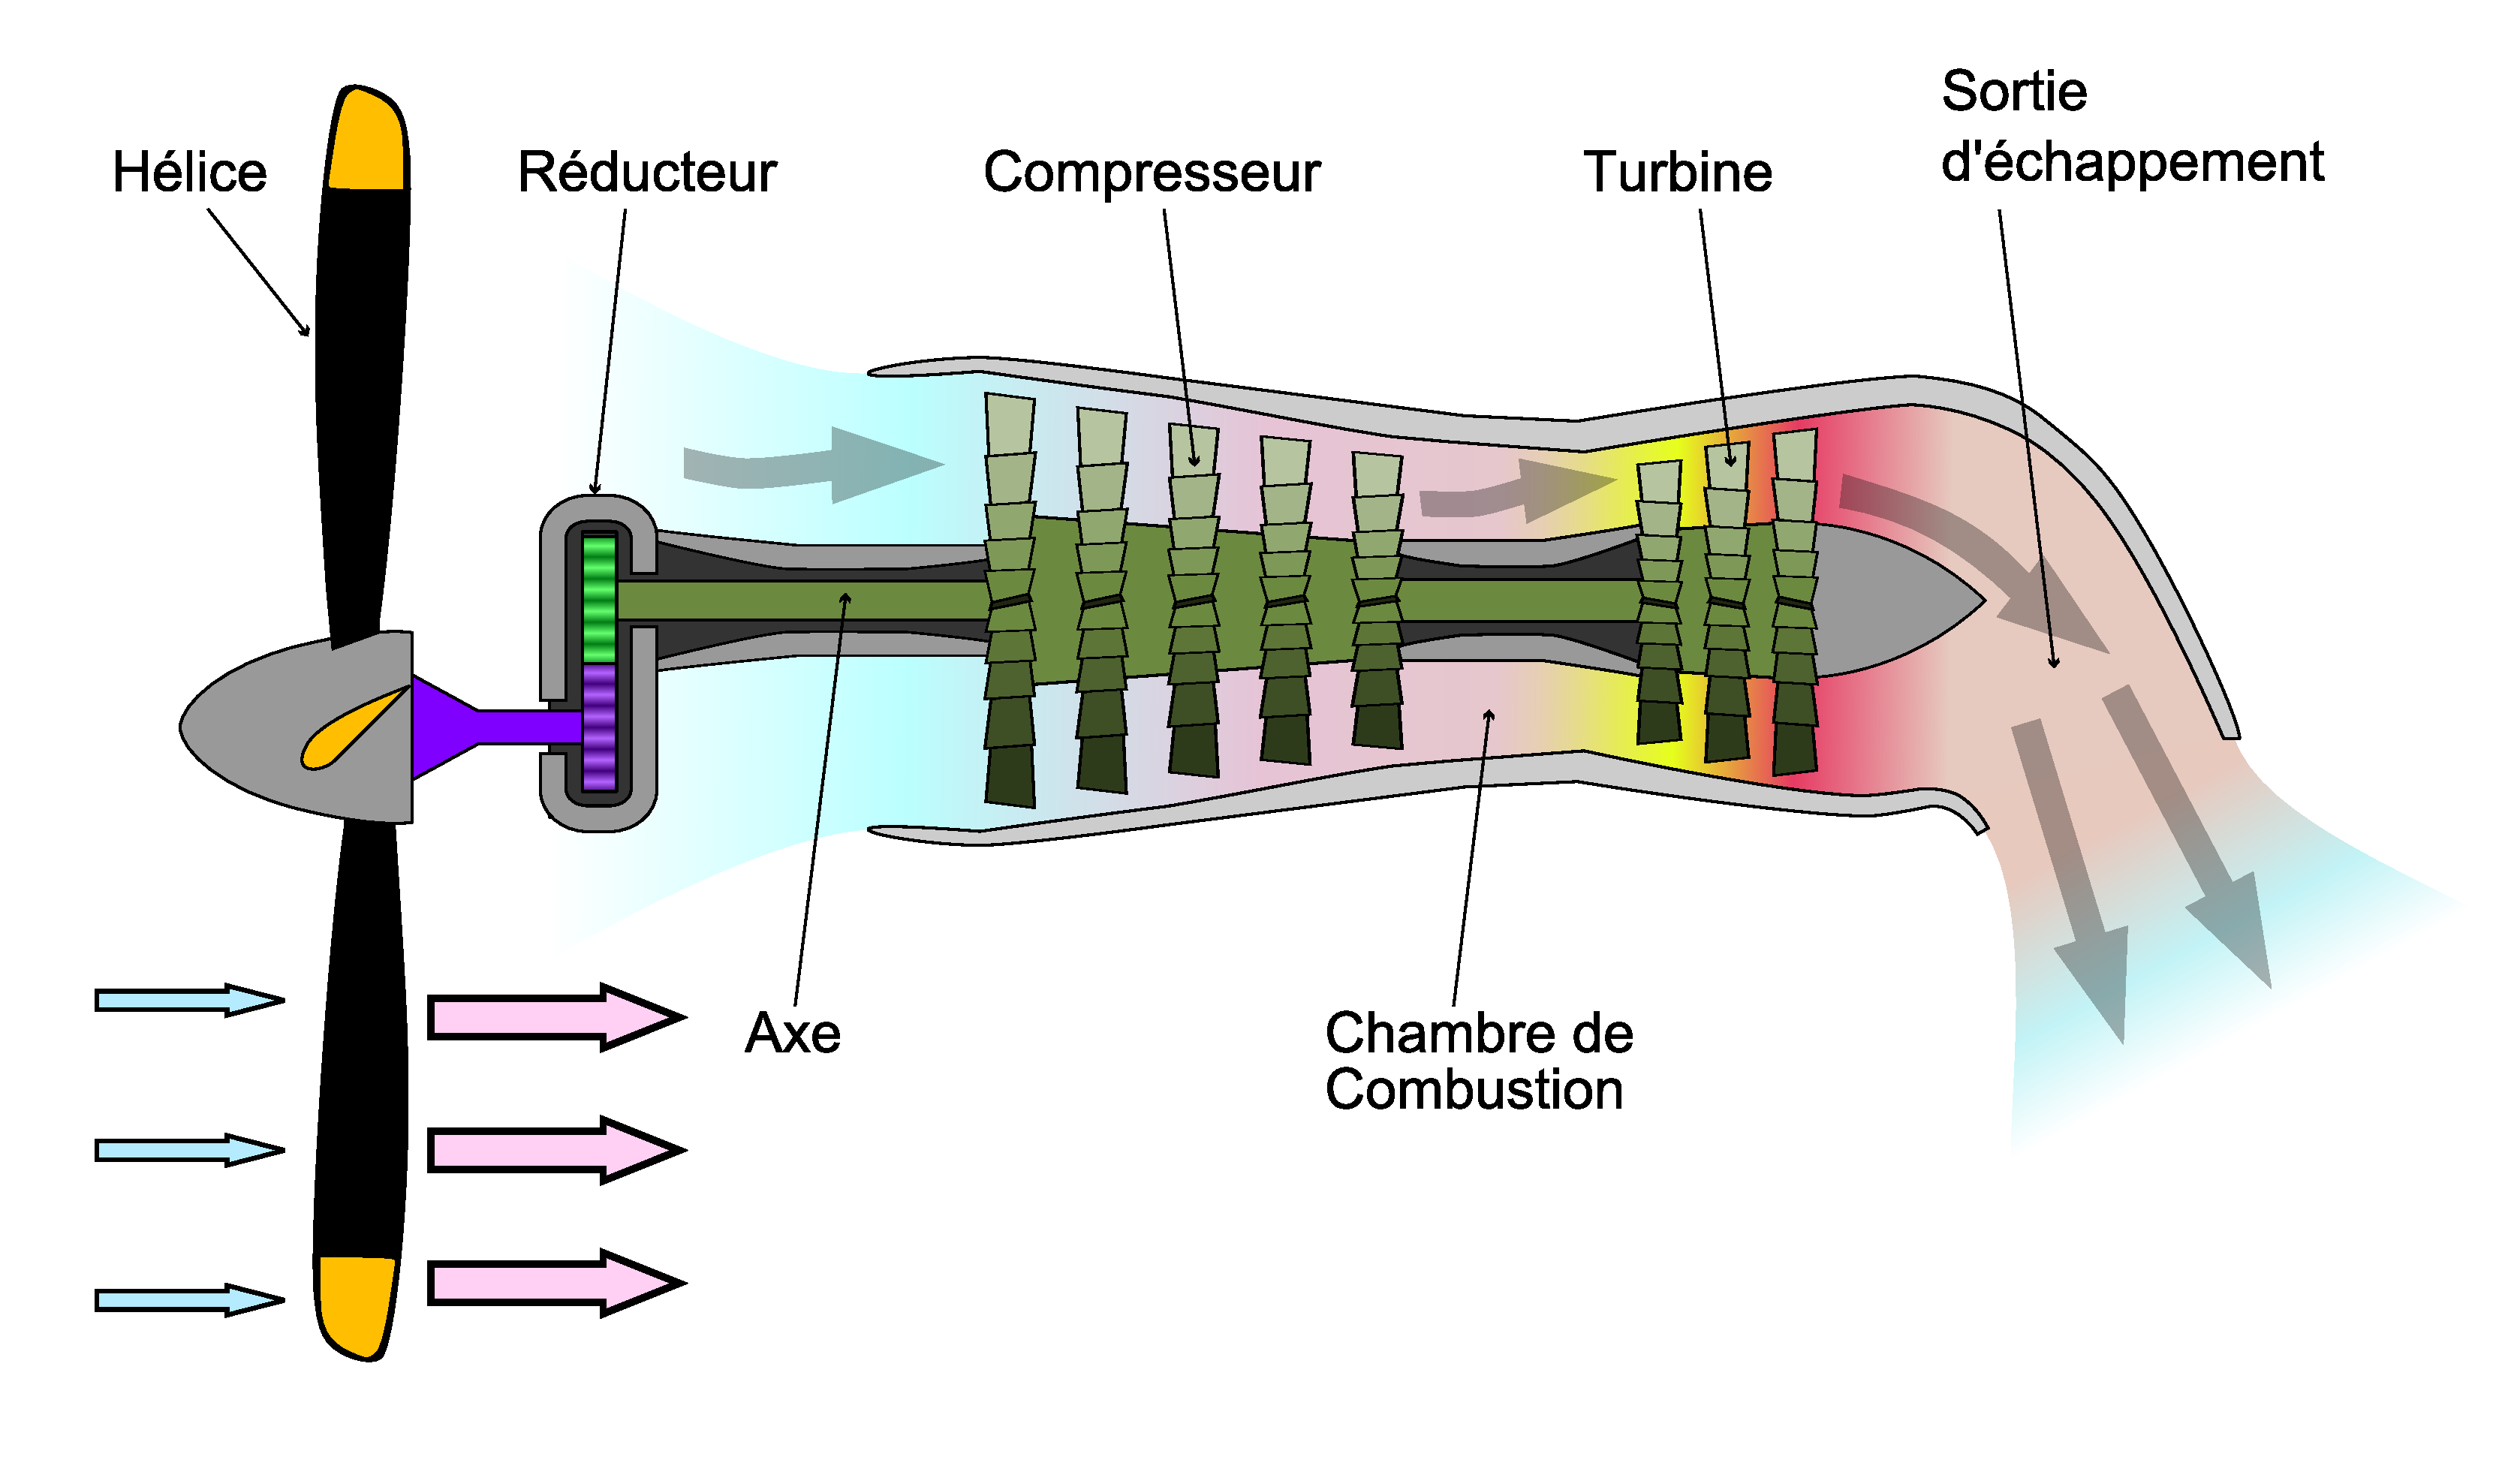
\includegraphics[width=0.82\textwidth]{01-EtudeAeronefs/img/turbomachines/turbopropulseur.pdf}
  	\legende{Schéma d'un turbopropulseur}{img:turbopropulseur}
	\end{figure}	
 \end{frame}
 
   \begin{frame}{Turbopropulseur}
	\begin{itemize}
		\item la propulsion par une hélice est plus économique que le turboréacteur aux faibles vitesses (jusqu'à 600-700 km/h)
		\item aussi fiable qu'un turboréacteur
		\item rapport puissance/poids compétitif par rapport aux moteur à explosion
	\end{itemize}
	
	\begin{columns}
  	\begin{column}{0.5\textwidth}
  	\begin{figure}[H]
  		\centering
    		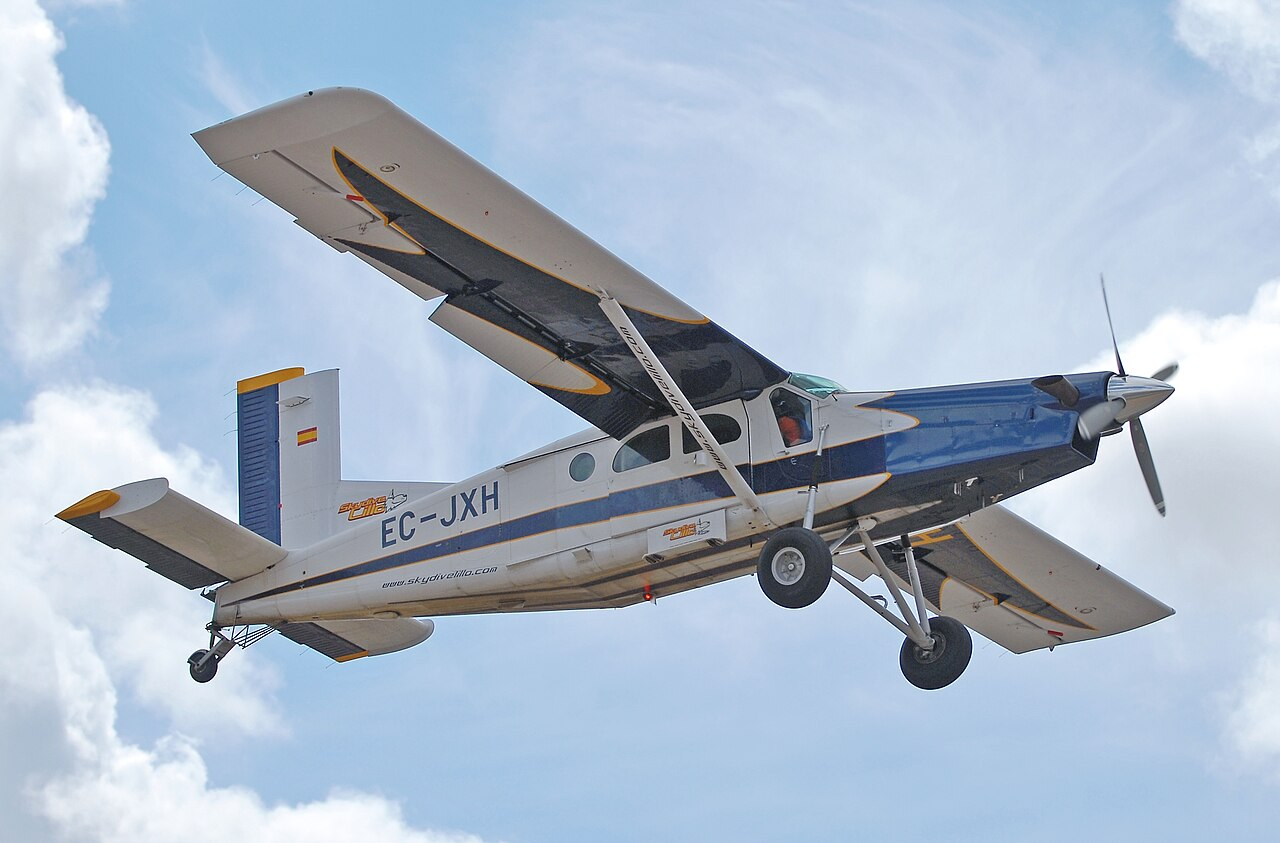
\includegraphics[width=0.5\textwidth]{01-EtudeAeronefs/img/Pilatus_PC-6.jpg}
  		\legende{Pilatus PC6 équipé d'un turbopropulseur P\&W PT6A-27, 131 kg, puissance 715 CV}{img:Pilatus_PC-6}
	\end{figure}	
  	\end{column}
  	\begin{column}{0.5\textwidth}
  	\begin{figure}[H]
  		\centering
    		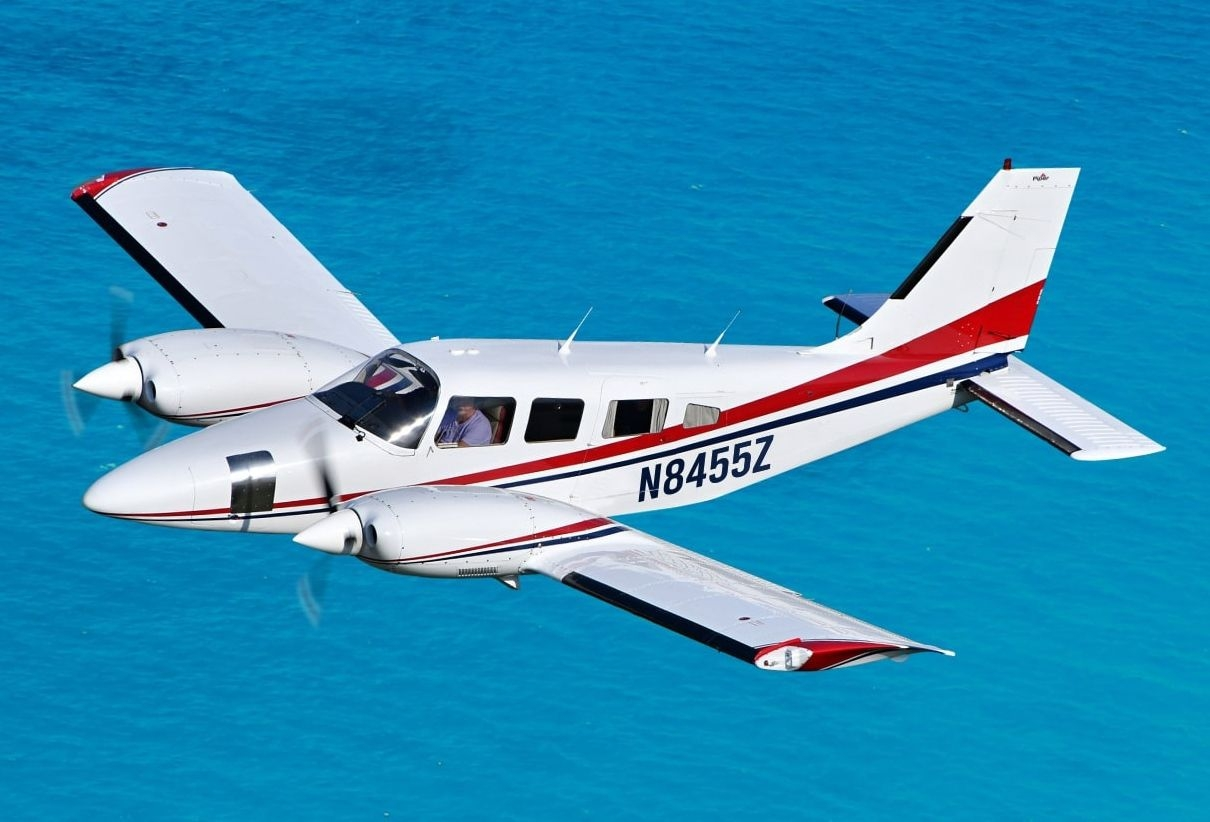
\includegraphics[width=0.5\textwidth]{01-EtudeAeronefs/img/Piper_PA-34.jpg}
  		\legende{Piper PA-34 équipé de moteurs à explosion Lycoming IO-360-C1E6, 139 kg, puissance 200 CV}{img:Piper_PA-34}
	\end{figure}	
  	\end{column}
  	\end{columns}
 \end{frame}
 
\section{Les hélices}
\begin{frame}{L'hélice \anglais{propeller}}
		Les hélices sont destinées à transmettre la puissance des moteurs pour mettre en mouvement les aéronefs. L'hélice propulse de l'air de l'avant vers l'arrière, et en réaction, l'aéronef est propulsé vers l'avant.
		
		\begin{figure}[H]
  		    		\centering
    		    		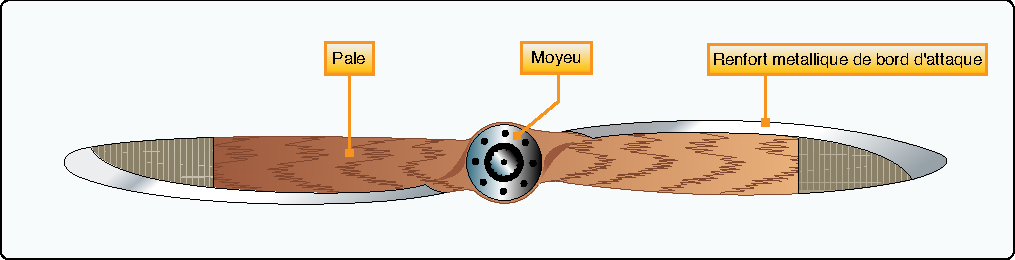
\includegraphics[width=0.8\textwidth]{01-EtudeAeronefs/img/heliceBois.pdf}
  		    		\legende{Une hélice en bois}{img:heliceBois}
	      	\end{figure}	
		
		Les hélices sont réalisées en bois, en aluminium forgé ou en composites, un assemblage de plusieurs matériaux.
\end{frame}

\begin{frame}{L'hélice - "vrillage" des pales}
	\begin{columns}
 		\begin{column}{0.35\textwidth}
 	     	\begin{figure}[H]
  		    		\centering
    		    		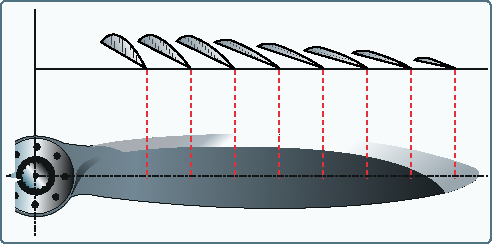
\includegraphics[width=0.8\textwidth,angle=90]{01-EtudeAeronefs/img/heliceAnglePale.pdf}
  		    		\legende{Succession des profils le long d'une pale}{img:heliceAnglePale}
	      	\end{figure}	
 		\end{column}
 		\pause
 		\begin{column}{0.65\textwidth}
 			\begin{figure}[H]
  		    		\centering
    		    		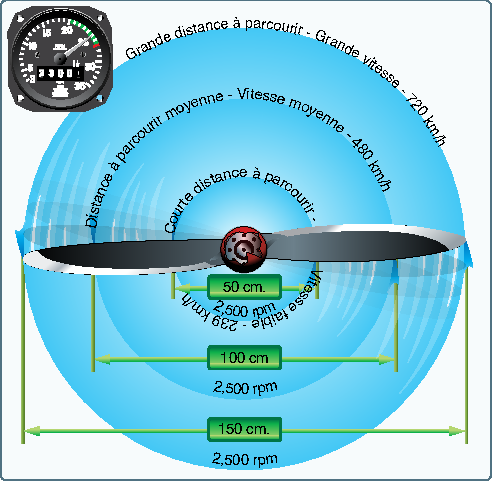
\includegraphics[width=0.7\textwidth]{01-EtudeAeronefs/img/heliceVitesseSection.pdf}
  		    		\legende{Vitesse en 3 points d'une pale}{img:heliceVitesseSection}
	      	\end{figure}	
 		\end{column}
	\end{columns}
\end{frame}

\begin{frame}{Calage d'une hélice}
	\begin{columns}
 		\begin{column}{0.35\textwidth}
 			\begin{figure}[H]
  		    		\centering
    		    		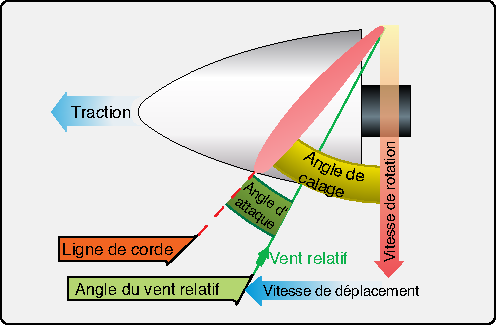
\includegraphics[width=1.1\textwidth]{01-EtudeAeronefs/img/heliceAerodynamique.pdf}
  		    		\legende{Calage d'une hélice}{img:heliceAerodynamique}
	      	\end{figure}	
 		\end{column}
 		\begin{column}{0.65\textwidth}
		L'angle que forme l'hélice avec l'axe de rotation détermine la quantité d'air que l'hélice envoie vers l'arrière. On appel cet angle le calage. \pause
		
		Sur une hélice monobloc, ce calage est fixe et déterminé à la fabrication. Il s'agit d'un compromis entre un calage faible, plus efficace au décollage, et un calage plus élevé, qui favorise la vitesse de croisière.
	     \end{column}
     \end{columns}
		
\end{frame}

\begin{frame}{Calage d'une hélice}
		Pour augmenter la performance d'une hélice, il existe des hélices dont le calage peut être modifié en vol : les hélices à calage variable. Ce système s'assimile aux vitesse d'une voiture ou d'un vélo.
		
		\begin{figure}[H]
  		    		\centering
    		    		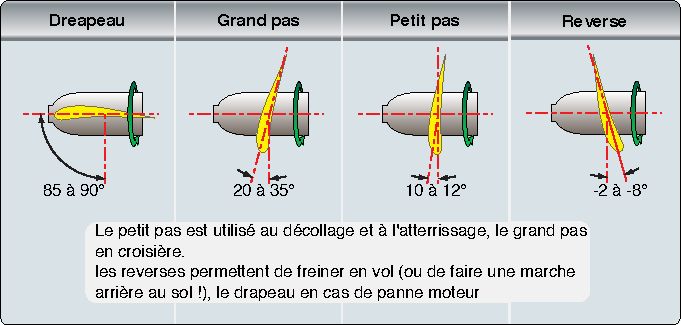
\includegraphics[width=0.8\textwidth]{01-EtudeAeronefs/img/heliceCalagePale.pdf}
  		    		\legende{Calages caractéristiques d'une hélice}{img:heliceCalagePale}
	      	\end{figure}	
		
		
\end{frame}
 
\appendix 
\section{QCM}
 \qmcBia{Étude des aéronefs}
{3}{Dans un moteur à 4 temps, la compression intervient après :}
{la combustion}
{la détente}
{l'admission}
{l'échappement}
{}

 \qmcBia{Étude des aéronefs}
{2}{Durant un cycle de fonctionnement d'un moteur à pistons (4 temps), le seul temps où le piston monte du point mort bas au point mort haut avec les soupapes fermées est le temps :}
{d'admission}
{de compression}
{de combustion-détente}
{d'échappement}
{}

\qmcBia{Étude des aéronefs}
{3}{Sur un avion certifié, un moteur à pistons contenant 4 cylindres est pourvu au total de :}
{2 bougies d'allumage}
{4 bougies d'allumage}
{8 bougies d'allumage}
{0 bougie d'allumage}
{}

\qmcBia{Étude des aéronefs}
{3}{\begin{figure}[H]
  		\centering
    		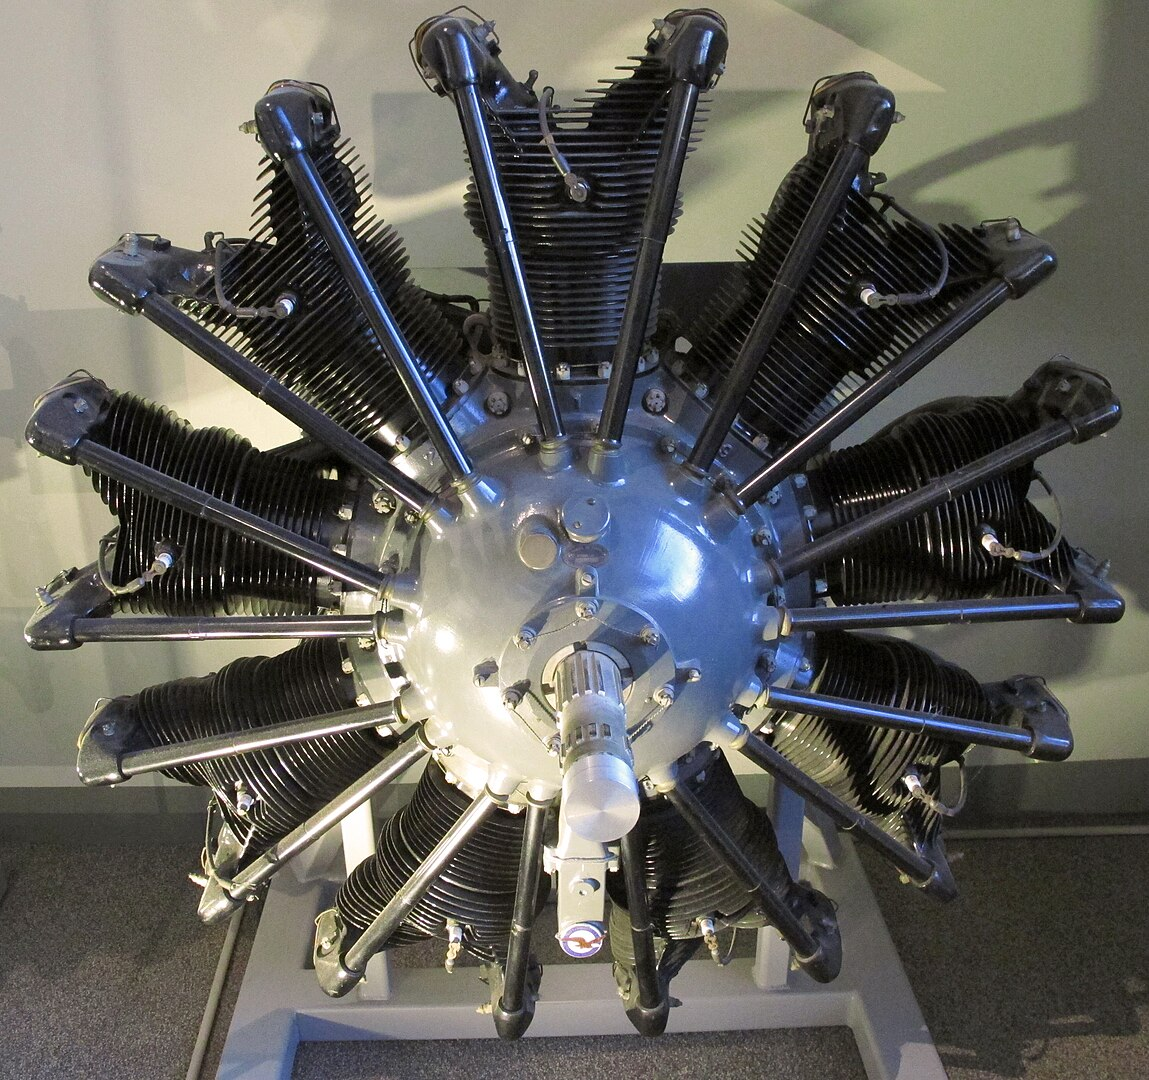
\includegraphics[width=0.2\textwidth]{01-EtudeAeronefs/img/PWWasp.jpg}
	\end{figure}	
	La disposition des cylindres de ce moteur est :}
{en ligne}
{en V}
{en étoile}
{à plat} 
{}

\qmcBia{Étude des aéronefs}
{4}{Un turbopropulseur}
{est un pulsoréacteur précédé d'un réducteur et d'une hélice}
{est un statoréacteur précédé d'un réducteur et d'une hélice}
{est un moteur à pistons équipé d'un turbocompresseur}
{est un turboréacteur précédé d'un réducteur et d'une hélice} 
{}


\qmcBia{Étude des aéronefs}
{3}{\begin{figure}[H]
  		\centering
    		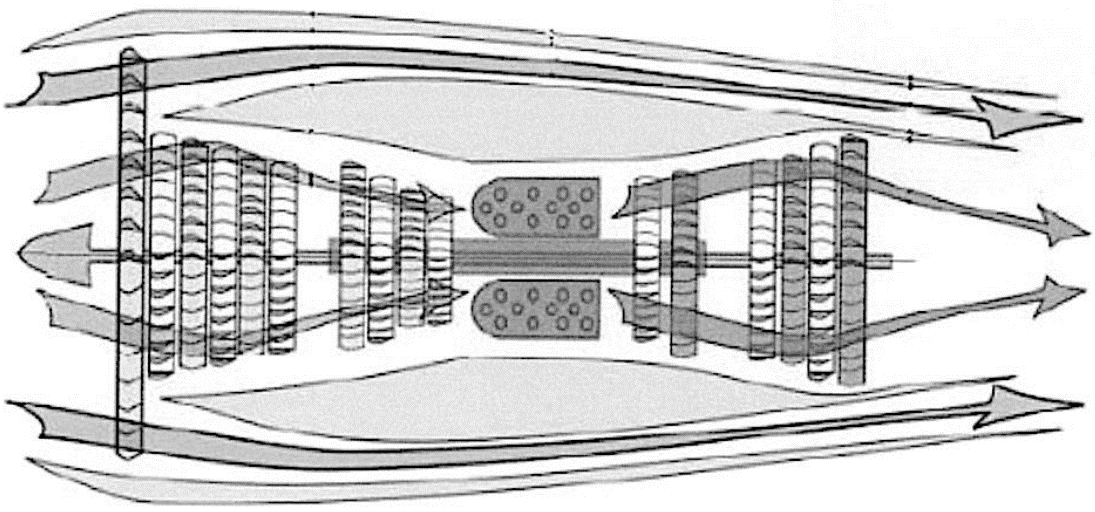
\includegraphics[width=0.4\textwidth]{imgPresentations/bia2024Q3.20.png}
	\end{figure}	
	Quel est le type de moteur de la photo ci-dessus ?}
{Turboréacteur double corps et simple flux}
{Turboréacteur simple corps et double flux}
{Turboréacteur double corps et double flux}
{Turboréacteur simple corps et simple flux} 

\qmcBia{Étude des aéronefs}
{2}{La présence d'un réchauffage de carburateur est nécessaire pour :}
{Améliorer son fonctionnement à froid}
{Pallier la formation de glace dans le venturi}
{Échauffer le mélange avant d'entrer dans les cylindres, et donc, améliorer sa combustion}
{Démarrer le moteur} 

\qmcBia{Étude des aéronefs}
{4}{Un turbopropulseur : }
{est un pulsoréacteur précédé d'un réducteur et d'une hélice}
{est un statoréacteur précédé d'un réducteur et d'une hélice}
{est un moteur thermique équipé d'un turbocompresseur}
{est un turboréacteur précédé d'un réducteur et d'une hélice}

\qmcBia{Étude des aéronefs}
{3}{Le petit pas de l'hélice à pas variable est utilisé pour :}
{l'atterrissage uniquement}
{le décollage uniquement}
{le décollage et l'atterrissage}
{le vol de croisière}

\qmcBia{Étude des aéronefs}
{1}{Vous volez avec un avion équipé d'une hélice "petit pas" c'est-à-dire à faible calage. Vous vous attendez à :}
{de bonnes performances au décollage au détriment des performances en croisière}
{de bonnes performances au décollage sans conséquence sur les performances en croisière}
{de bonnes performances en croisière au détriment des performances au décollage}
{de mauvaises performances au décollage ainsi qu’en croisière}

 
\ifdefined\activerbibliobeamer
\begin{frame}[allowframebreaks]
\frametitle{Bibliographie}
\printbibliography
%\nocite{*}
\end{frame}
\fi 
 
\end{document}
